\chapter{Cosmic muon detection using an assembled Si(Li) tracker module} \label{ch3}

The following Chapter describes the test setup and the consequent experimental results concerning the search and detection of cosmic muons by means of an assembled Si(Li) tracker module of the GAPS experiment.

\par
The Chapter is structured as follows. Initially, the physical background concerning cosmic muons, their nature and detection possibilities on planet Earth is given. Next, a description of the test setup adopted to carry out the measurements is provided, which is comprised of an assembled Si(Li) tracker module and an ArduSiPM ionising radiation detector, used as a trigger for the readout electronics. Finally, the experimental results obtained from the detection are reported, with an explanation of their usefulness in the context of flight item characterisation. This Section also reports the results obtained during the characterisation activity that has been performed on the fully assemble Si(Li) tracker module.

%-------------------------------------------------------------------------------
%   Cosmic muons
%-------------------------------------------------------------------------------

\section{Cosmic muons}

Cosmic rays are intense particles that continually rain through the Earth's atmosphere, with a portion of them penetrating the surface at relativistic speeds. Cosmic rays provide a homogeneous background ionising radiation that showers on the Earth's atmosphere at a rate of around 1000 collisions per square meter every second \cite{uretsky_1997_penetration}. The sun or more exotic occurrences like supernovae and black holes can be the source of these particles. Most of the energy coming from cosmic rays reaches the Earth's surface in the form of muon kinetic energy.

\par
Muons ($\mu^{-}$ and $\mu^{+}$) are elementary particles similar to electrons, but with much greater mass. They belong to the lepton family \cite{klapdorkleingrothaus_2018_lepton} and form as a result of interactions between very energetic cosmic rays and the nuclei of atmospheric particles. They are the product of pion decay ($\pi^{-}$ and $\pi^{+}$). The muons formed in the atmosphere may infiltrate the Earth's surface for hundreds of meters due to their ultra-relativistic character, which stems from the fact that these particles have a speed near to that of light. The flux of these particles may be distinguished adequately with a scintillator detection setup, as used in this experiment.

\par
When cosmic rays collide with the atmosphere, they can cause a particle \textit{shower}, which is a series of events that alter the character of the entering primary cosmic rays in other particles \cite{bonomi_2020_applications}. In a medium such as air, the particle shower has a hadronic core that serves as a source for electromagnetic subshowers. \hyperref[figCosmicRay]{Figure \ref{figCosmicRay}} shows an illustration of cosmic rays interacting with the atmosphere, where the air shower effect is evident.

\begin{figure}[h!]
    \centering
    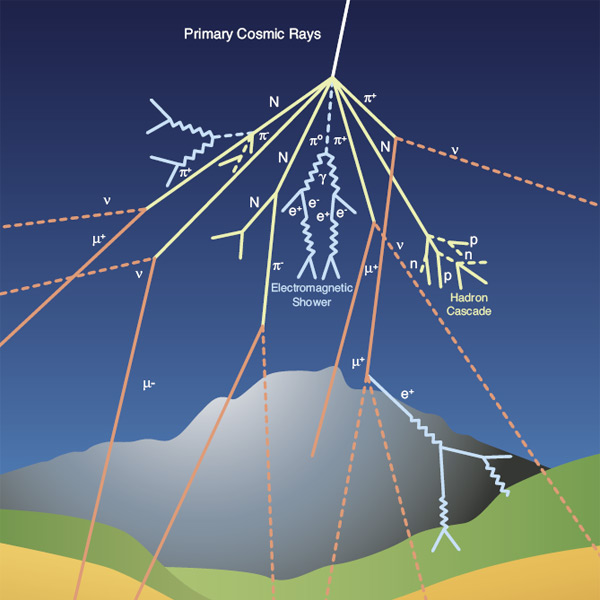
\includegraphics[width=0.65\textwidth]{Images/chap3/cosmic_ray.jpg}
    \caption{A diagram of cosmic rays interacting with the atmosphere and producing secondary particles. \cite{marzena_2017_cms}}
    \label{figCosmicRay}
\end{figure}

\par
Cosmic muons, on the other hand, have a mean lifetime of around \SI{2}{\micro\second} and may reach the Earth's surface at the speed of light. All of the particles in the air shower are collectively referred to as \textit{secondary cosmic rays}. Pacini, Hess, and other physicists discovered them around the beginning of the twentieth century while studying the electric conductivity of air. They eventually realised that, in the words of Pacini, \textit{``a sizeable cause of ionisation exists in the atmosphere, originating from penetrating radiation, independent of the direct action of radioactive substances in the crust''} \cite{deangelis_2012_domenico, alessandrodeangelis_2012_lenigma}. It was Millikan that for the first time, after these experiments, called this extraterrestrial radiation \textit{cosmic rays}.  The cosmic rays, after discovery and for a few decades before the takeover of particle accelerators, have been the main source for the early development of particle physic.

\par
The flux of muons with a momentum greater than \SI{1}{\giga\electronvolt} at sea level has been measured to be around \SI[parse-numbers=false]{(0.94 \pm 0.12) \times 10^{-2}}{\cm^{-2}.sr^{-1}.s^{-1}} \cite{tanabashi_2018_review, allkofer_1975_the}. It can be said that 10 000 of muons per minute and per square (horizontal) meter, or alternatively \SI{\approx 170}{\hertz\per\meter^{2}}, hit the ground. On average about 600 of them cross a human body every minute. Another easy to remember rule of thumb is that 1 muon per second intercepts the palm of a hand. These are indicative values, since the flux depends on many variables such as altitude, solar activity, Earth and other factors. The average energy of muons at sea level is comprised between \SI{3}{\giga\electronvolt} and \SI{4}{\giga\electronvolt} and the flux is maximum
at the zenith (vertical direction) and it scales approximately with $\cos^{2}(\theta)$, $\theta$ being the angle with respect to the vertical.

%-------------------------------------------------------------------------------
%   Experiment setup
%-------------------------------------------------------------------------------

\section{Experiment setup}

This Section provides a description of the setup used for the detection of cosmic muons through the joint use of the ArduSiPM ionising radiation detector and a fully assembled Si(Li) tracker module. Tests were conducted using the same setup described in \hyperref[sec21]{Section \ref{sec21}} and shown in \hyperref[figFEBtest1]{Figure \ref{figFEBtest1}}, the only difference being that instead of testing a FEB without Si(Li) detectors, in this case a complete module with 4 Si(Li) detectors was tested. The complete experiment setup is shown in more detail in \hyperref[figModuleSetup]{Figure \ref{figModuleSetup}}.

\par
In order to carry out the tests on the module, the latter was powered by means of two instruments:

\begin{itemize}
    \itemsep0em
    \item A Keysight N6705C DC Power Analyser providing both analog and digital supply voltages to the FEB, in the same configuration described in \hyperref[sec21]{Section \ref{sec21}} and shown in \hyperref[figKeysightFEB]{Figure \ref{figKeysightFEB}}.
    \item A CAEN HiVolta DT1415ET high voltage power supply used in order to bias the Si(Li) detectors with a negative DC voltage of \SI{-250}{\volt}. 
\end{itemize}

\noindent
Both instruments were controlled by means of a specially developed Python application in order to ensure the correct switch-on and switch-off sequence, which has to be performed by first switching on the power supply to the readout electronics via the Keysight N6705C DC Power Analyser and then the CAEN HiVolta to supply the \SI{-250}{\volt} biasing voltage to the Si(Li) detectors in a time interval of at least \SI{1}{\milli\second} and with a maximum increase of \SI{4}{\volt/\second} in order to avoid damage to the Si(Li) detectors. The switch-off sequence must be carried out in the exact reverse order with the same time constraint and voltage slope. The code can be found on GitHub at the following \href{https://github.com/lucaghislo/GAPS_module_setup}{\underline{link}}.

\begin{figure}[h!]
    \centering
    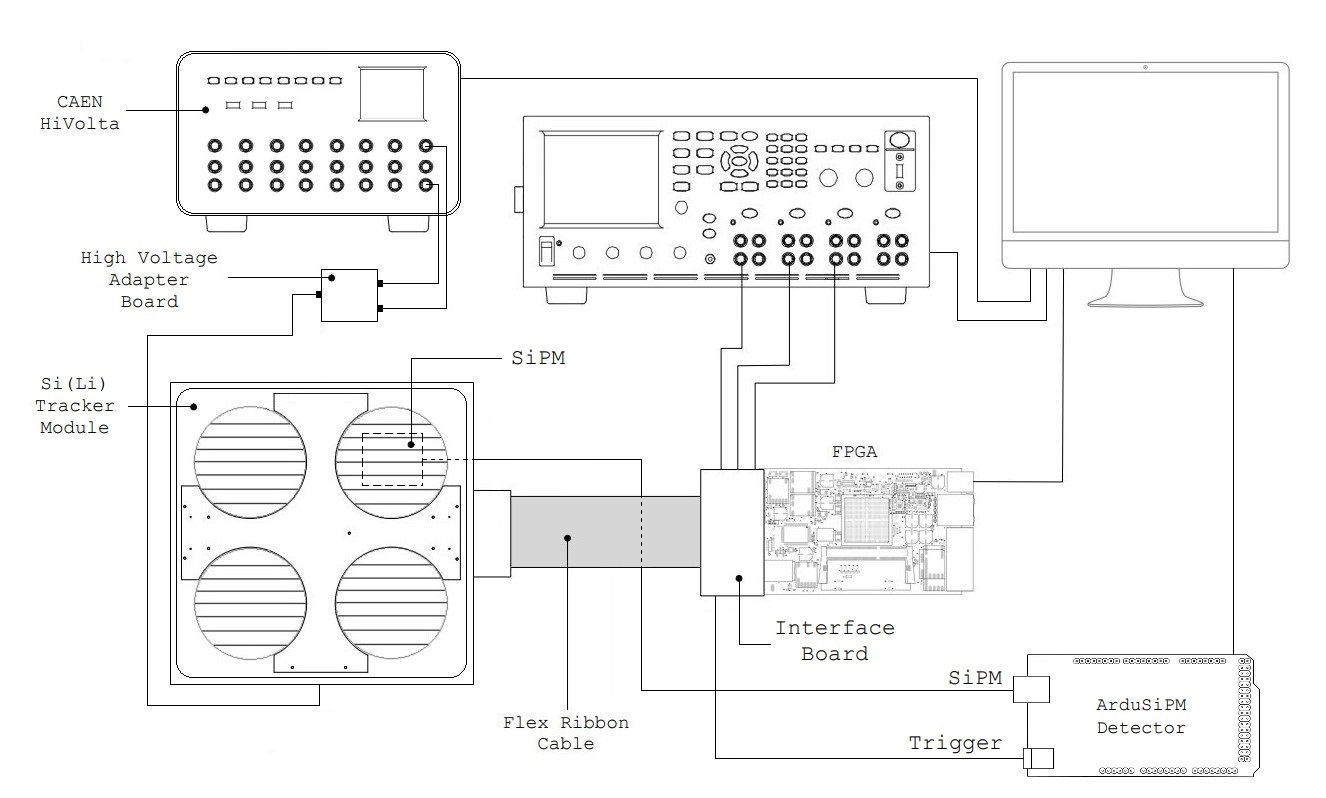
\includegraphics[width=0.99\textwidth]{Images/chap3/test_setup_MODULE.jpg}
    \caption{Complete muon detection experiment setup.}
    \label{figModuleSetup}
\end{figure}

\par
The tests were carried out in a climate chamber, model ACS DY110, at a constant temperature of \SI{-40}{\celsius} and \SI{10}{\percent} relative humidity. The transition from room temperature to \SI{-40}{\celsius} and vice versa was carried out with a decrease of \SI{0.5}{\celsius/\second} in order to avoid sudden temperature changes and consequent damage to the Si(Li) detectors, as well as the formation of condensation.

\par
In order to connect the high voltage lines coming from the CAEN HiVolta to the FEB, a specifically built adapter board, shown in \hyperref[figHiVoltAdapterBoard]{Figure \ref{figHiVoltAdapterBoard}}, has been developed in order to connect the negative and positive terminals of one channel of the CAEN HiVolta through two separate high voltage cables into a single one connected to the FEB. This adapter board presents on one end a BNC connector and on the other a HIROSE MDF51SU high voltage connector to be hooked up to the respective HIROSE MDF51SY housing on the FEB. Both connectors are shown in \hyperref[figHVPSconn]{Figure \ref{figHVPSconn}}.

\par


\begin{figure}[h!]
    \centering
    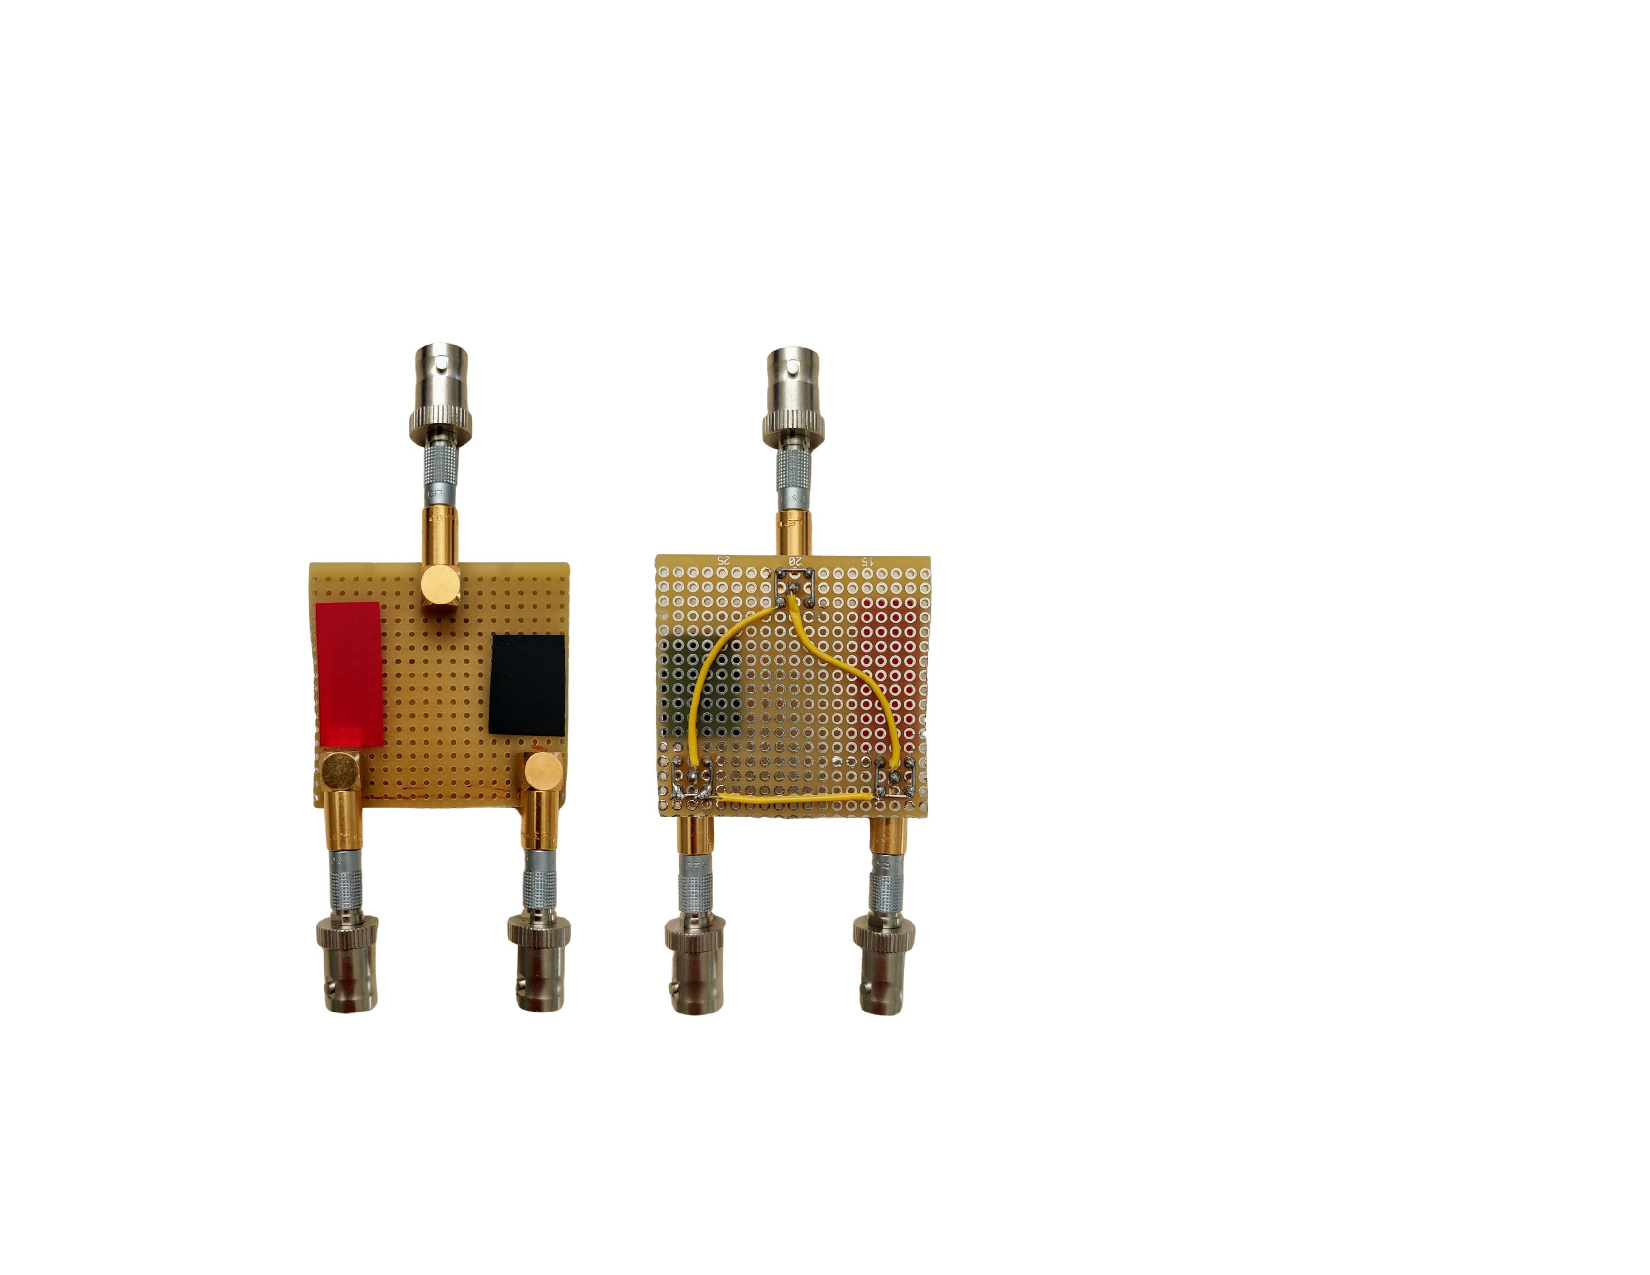
\includegraphics[width=0.45\textwidth]{Images/chap3/hivoltage_adapter_board.pdf}
    \caption{Top (on the left) and bottom (on the right) view of the purpose built high voltage adapter board designed to connect the CAEN HiVolta high voltage power supply to the Si(Li) tracker module.}
    \label{figHiVoltAdapterBoard}
\end{figure}

\begin{figure}[h!]
    \centering
    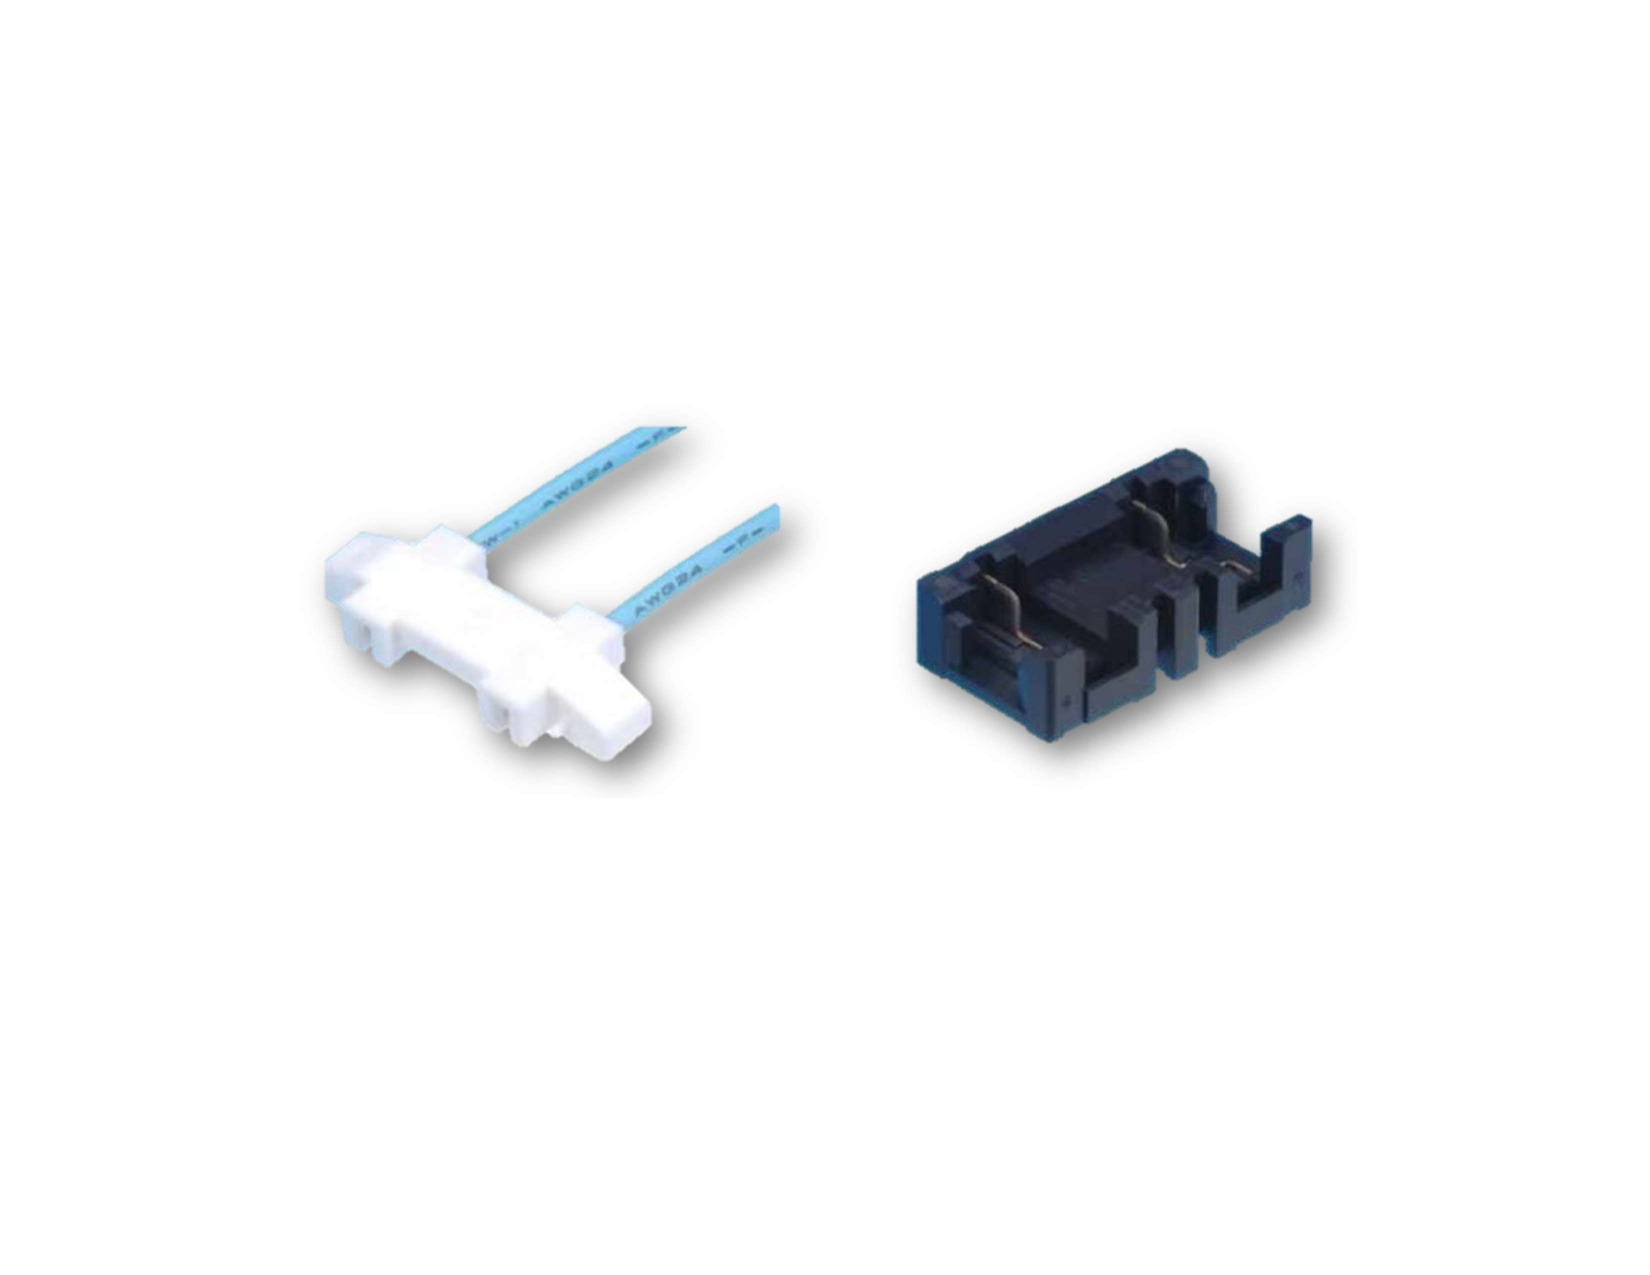
\includegraphics[width=0.45\textwidth]{Images/chap3/connectors_high_voltage.pdf}
    \caption{HIROSE high voltage connector model MDF51SU on the left and model MDF51SY on the right.}
    \label{figHVPSconn}
\end{figure}

%-------------------------------------------------------------------------------

\subsection{ArduSiPM}
\label{secArduSiPM}
\textit{ArduSiPM} is a complete ionising particle detection and data acquisition system consisting of an open source Arduino Due board, a purpose-built shield connected to an Arduino 2 board called \textit{ArduSiPM Shield} and a scintillator connected to a Silicon PhotoMultiplier (SiPM) \cite{bocci_2015_particle}. 

\par
The scintillator was placed below one of the Si(Li) detectors, at a distance of between 4 and \SI{5}{\cm}. Due to the small size of the scintillator, measuring \SI{5}{\cm} on each side, it was not possible to cover the entire surface of the circular detector. Therefore, the scintillator was placed below the central part of channels 16, 17, 18 and 19, like shown in \hyperref[figScintillatorSiLi]{Figure \ref{figScintillatorSiLi}}.

\begin{figure}[h!]
    \centering
    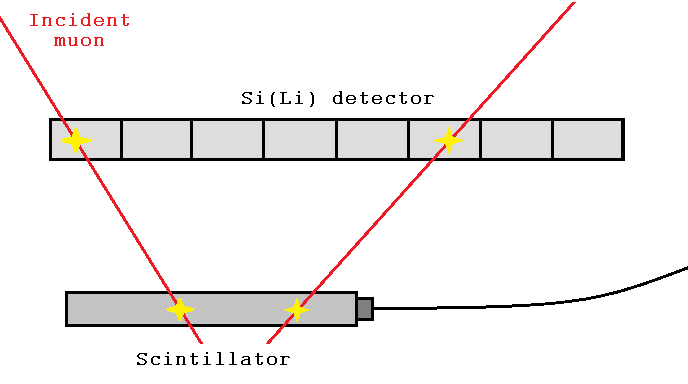
\includegraphics[width=0.55\textwidth]{Images/chap3/scintillator_sensor_detail.png}
    \caption{Scintillator placement with respect to the Si(Li) detector.}
    \label{figScintillatorSiLi}
\end{figure}

\par
The transit of an ionising particle through the scintillator produces a signal in the photomultiplier that is processed by the electronics on the board. The complete device assembly is shown in \hyperref[figArduiSiPM]{Figure \ref{figArduiSiPM}}.

\begin{figure}[h!]
    \centering
    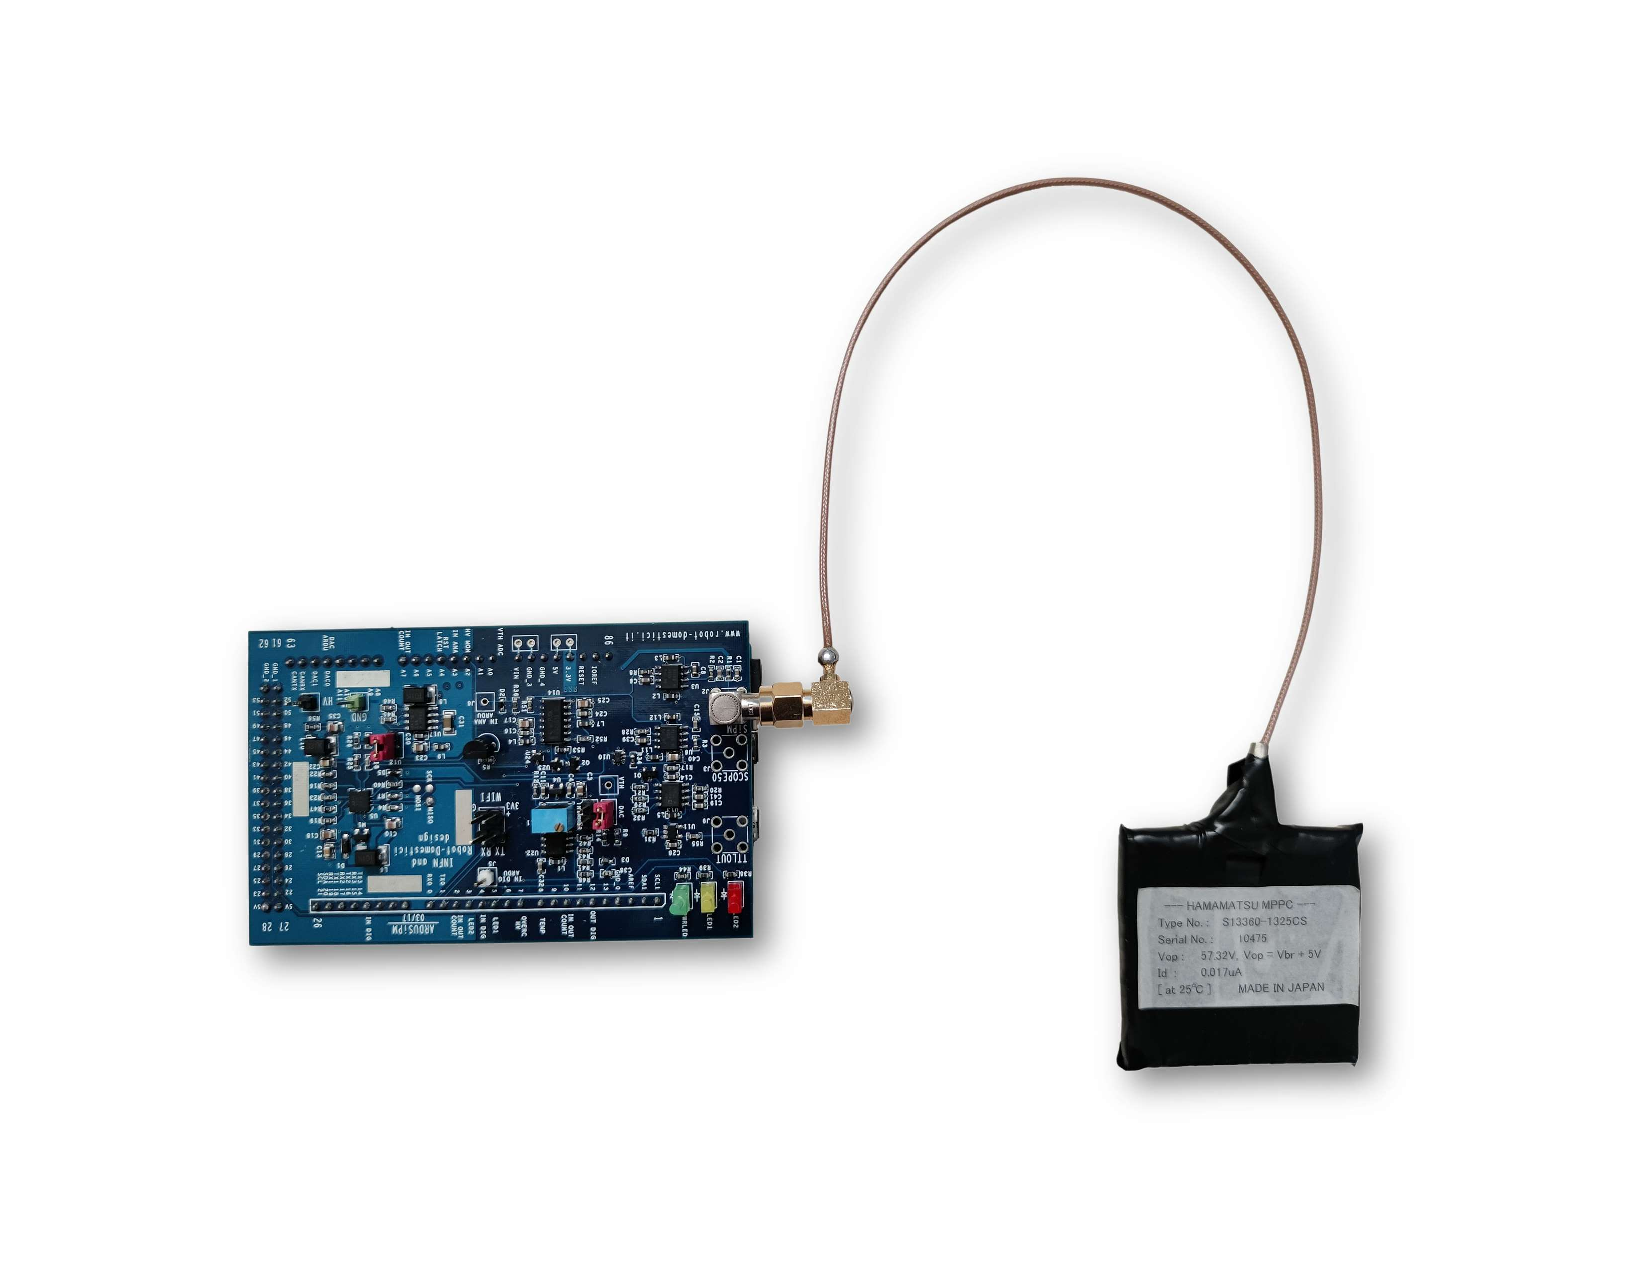
\includegraphics[width=0.65\textwidth]{Images/chap3/ardusipm_cropped.pdf}
    \caption{Picture of the ArduSiPM ionising particle detection and data acquisition system. It is possible to distinguish the ArduSiPM data acquisition board on the left and the detector module consisting of a scintillator and a photomultiplier on the right.}
    \label{figArduiSiPM}
\end{figure}

The ArduSiPM shield is installed above the Arduino Due board, which takes care of acquiring data and powering it. The shield electronics, on the other hand, is responsible for powering the photomultiplier and taking readings from it. Specifically, this board consists of the following components.

\begin{itemize}
    \itemsep0em
    \item A \textit{DC/DC converter} in the form of a boost converter capable of generating a DC output voltage between 30 and \SI{100}{\volt} needed to power the photomultiplier. The converter takes as input a voltage of \SI{5}{\volt} supplied directly from the Arduino Due's power supply.
    \item A \textit{fast low-noise amplifier} required in order to take the signal from the photomultiplier and adapt it to the reading range of the Arduino Due's ADC, which is responsible for counting events in the form of particles entering the photomultiplier.
    \item A \textit{fast discriminator} used to recognise above-threshold pulses from the photomultiplier. The output of this block is directly fed into the internal counter of the Arduino Due in order to count the photomultiplier interaction events.
    \item A \textit{peak detector}, i.e. a circuit built with the purpose of maintaining the peak voltage read out by the photomultiplier. The latter switches very quickly, so this circuit block is designed to be very rapid in detecting peaks at very close time intervals.
\end{itemize}

\par
The ArduSiPM device was used as a trigger for the readout electronics of the Si(Li) tracker module used in the experiment. For this purpose, the ArduSiPM Shield board provides a terminal on the board named \texttt{TTLOUT}, on which a signal of the type shown in \hyperref[figArduiSiPMtrigger]{Figure \ref{figArduiSiPMtrigger}} is provided when the silicon photomultiplier registers an interaction event.

\begin{figure}[h!]
    \centering
    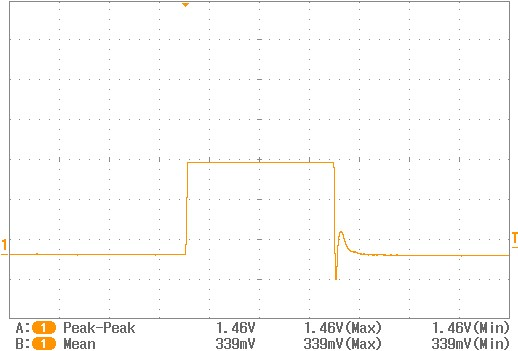
\includegraphics[width=0.53\textwidth]{Images/chap3/SCRN0097_crop.jpg}
    \caption{ArduSiPM trigger signal measured with a LeCroy Wavejet 314-A oscilloscope.}
    \label{figArduiSiPMtrigger}
\end{figure}

\noindent
An \textit{SMA} connector was installed on this terminal in order to connect the board to the trigger input of the interface board, visible in \hyperref[figModuleSetup]{Figure \ref{figModuleSetup}}. The connection between the photomultiplier and the board was made via a 2m-long \textit{Lemo} coaxial cable with a delay of \SI{10}{\nano\second}. On the other hand, the connection between the board and the trigger input of the interface board was realised with a \SI{1}{\meter} \textit{Lemo} coaxial cable with a \SI{5}{\nano\second} delay.

\par
The device is programmed via a specially developed firmware (version \texttt{2.1.5} is used) that allows data from the scintillator to be read via a USB connection to a PC via the serial interface of the Arduino IDE software used for programming. Additional software is also available, called \textit{ArduSiPM Acquisition Tool}, which allows data to be read and displayed on the screen in the form of graphs. It also allows to set some operating parameters and to monitor the serial communication. The software also makes it possible to carry out data acquisitions with tunable time duration, then exporting them in \texttt{csv} format.

\par
An important feature of the firmware flashed on the device is the possibility of setting various detector parameters directly from the serial interface, using a predefined set of commands \cite{bocci_2022_ardusipm}. Those of interest for the purposes of the experiment are the detection threshold, the acquisition frequency and the output data format.

%-------------------------------------------------------------------------------

\subsection{Si(Li) tracker module}
\label{siliModule}
\par
As can be appreciated in \hyperref[figSILImodule]{Figure \ref{figSILImodule}}, the complete Si(Li) tracker module comprises the following components, as discussed in \hyperref[ch2]{Chapter \ref{ch2}}.

\begin{itemize}
    \itemsep0em
    \item A front-end board, presented in \hyperref[sec21]{Section \ref{sec21}}, which in the specific case of module No. \texttt{238}, is FEB No. \texttt{F202I} from the Italian production.
    \item Two front-end board shields, described in \hyperref[secShield]{Section \ref{secShield}}, installed above the FEB by means of screws. Each module involves the use of one type A and one type B shield, that in this case are No. \texttt{S019AP} and No. \texttt{S019BP}.
    \item A metal scaffold placed centrally to the module above the FEB, which makes up the metal frame in which the module is housed.
    \item A thermal pad, not visible in the figure, placed between the FEB and the metal frame in order to act as a heatsink for the ASIC and guarantee cooling by means of a specially designed cooling system.
    \item Four circular Si(Li) detectors, each divided into 8 strips and connected via wire bonding to the FEB.
\end{itemize}

\begin{figure}[h!]
    \centering
    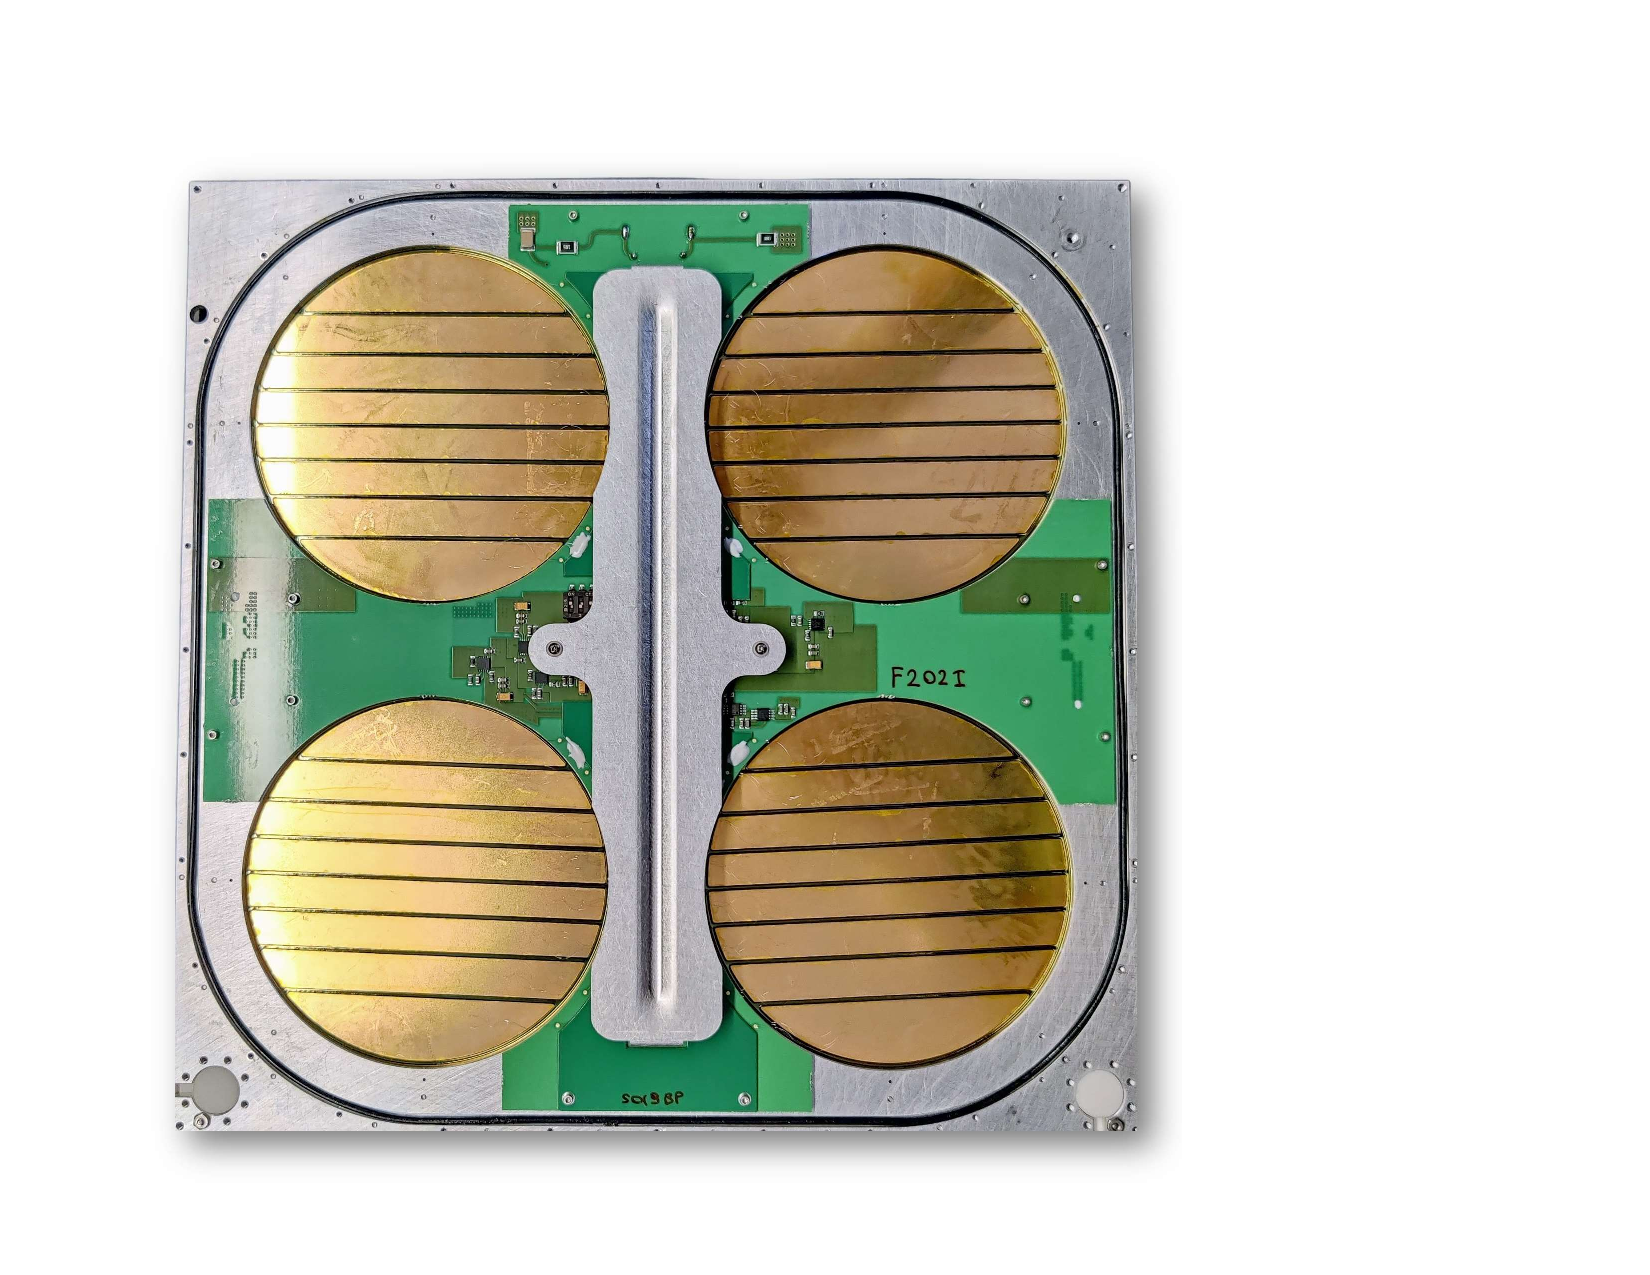
\includegraphics[width=0.6\textwidth]{Images/chap3/GAPS_module.pdf}
    \caption{GAPS Si(Li) tracker module No. \texttt{238} mounting the FEB No. \texttt{F202I} from the Italian production.}
    \label{figSILImodule}
\end{figure}

\par
The fully assembled tracker module shown in \hyperref[figSILImodule]{Figure \ref{figSILImodule}}, being equipped with four Si(Li) detectors, must be kept in a humidity-controlled environment, in order to avoid damage to the detectors. To do this, a portable microcontroller platform, called \textit{Winter}, developed by the Microelectronics Laboratory of the University of Bergamo and shown in \hyperref[figWinterBattery]{Figure \ref{figWinterBattery}}, was used, as it is equipped with multiple environmental sensors, including an hygrometer, a thermometer and a barometer. 

\begin{figure}[h!]
    \centering
    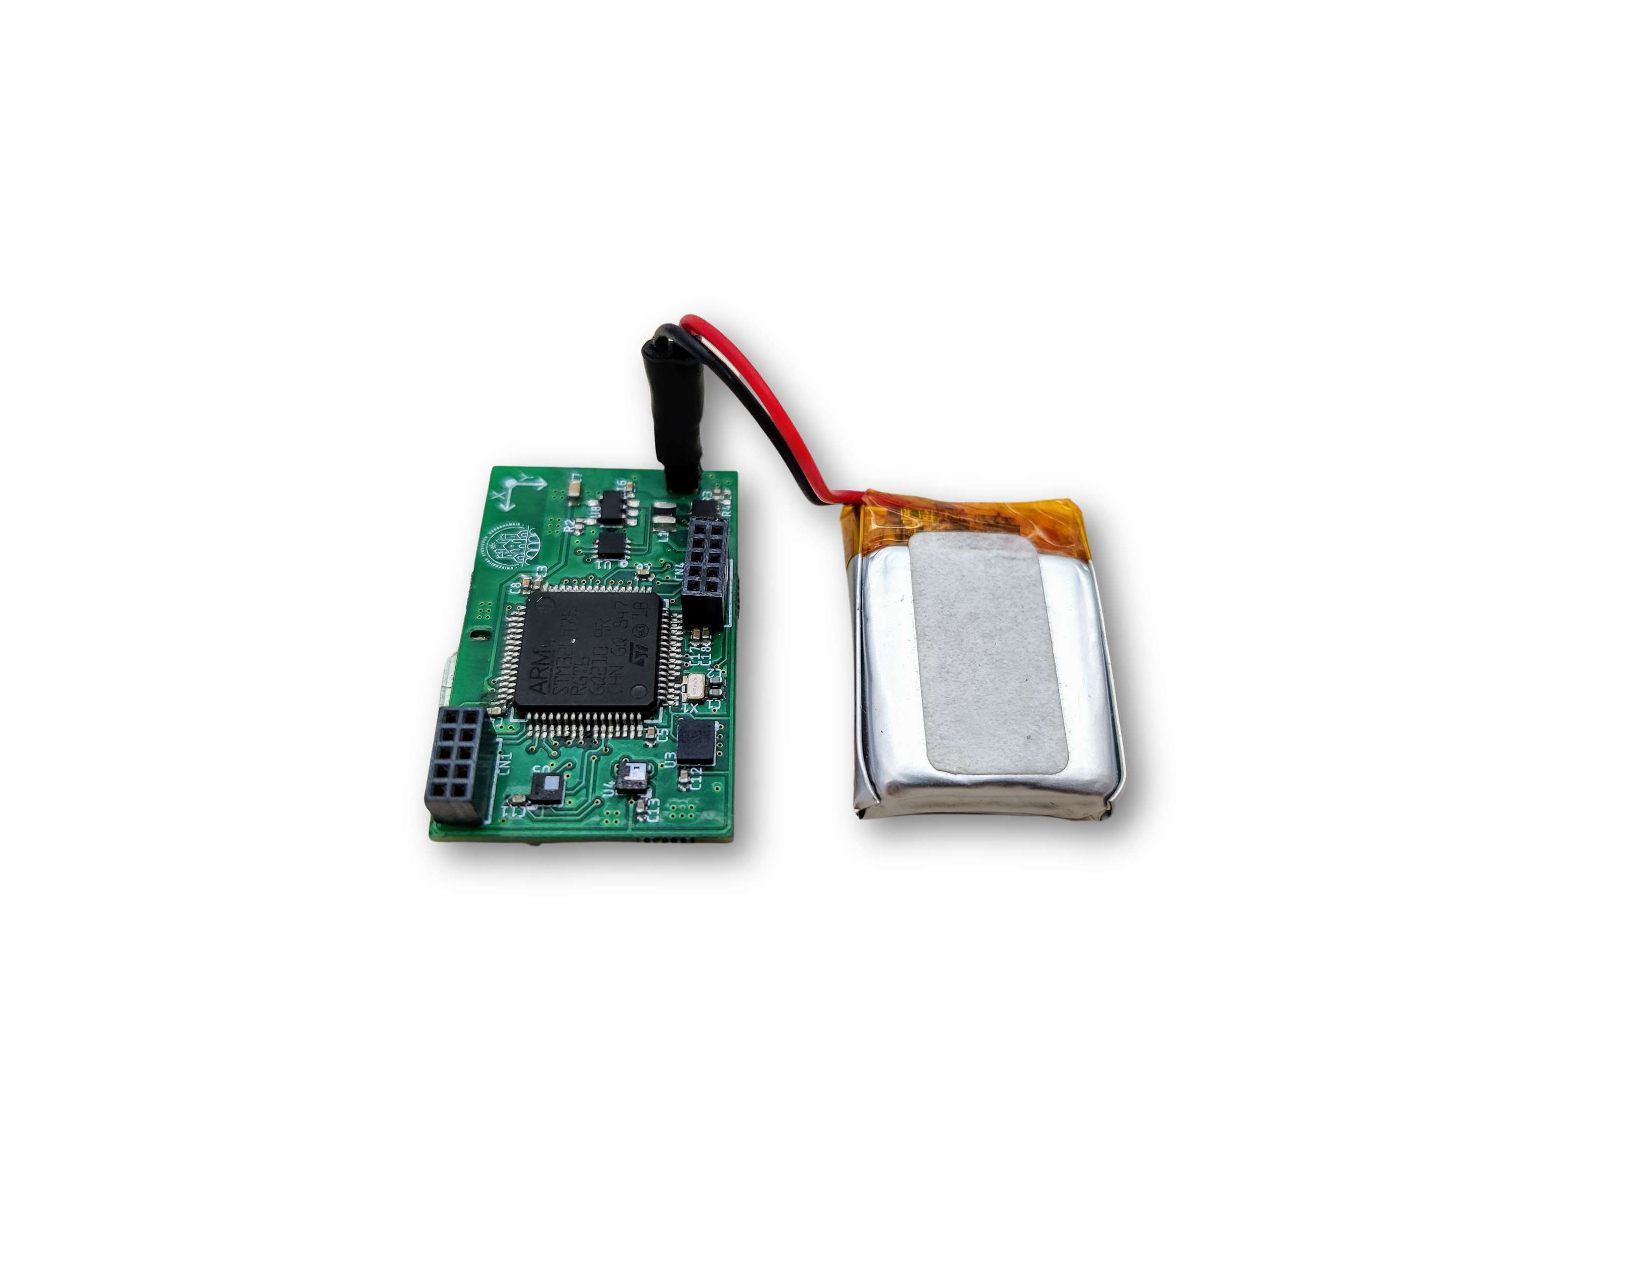
\includegraphics[width=0.4\textwidth]{Images/chap3/winter_battery.pdf}
    \caption{\textit{Winter} platform connected to a \SI{3.7}{\volt} \SI{240}{\milli\ampere h} lithium-ion battery.}
    \label{figWinterBattery}
\end{figure}

\par
The latter was placed together with the tracker module inside an airtight case in which desiccant bags were located, thus guaranteeing a low level of humidity and preventing damage to the Si(Li) detectors. The device, equipped with a Bluetooth Low Energy (BLE) v4.1 connection, was used to transmit humidity data at regular intervals, 24 hours a day, to a Raspberry Pi on which a Python script was run in order to acquire the values and save them to a file in \texttt{csv} format. The code can be found on GitHub at the following \href{https://github.com/lucaghislo/winter_enviroment_monitor}{\underline{link}}. 

\begin{figure}[h!]
    \centering
    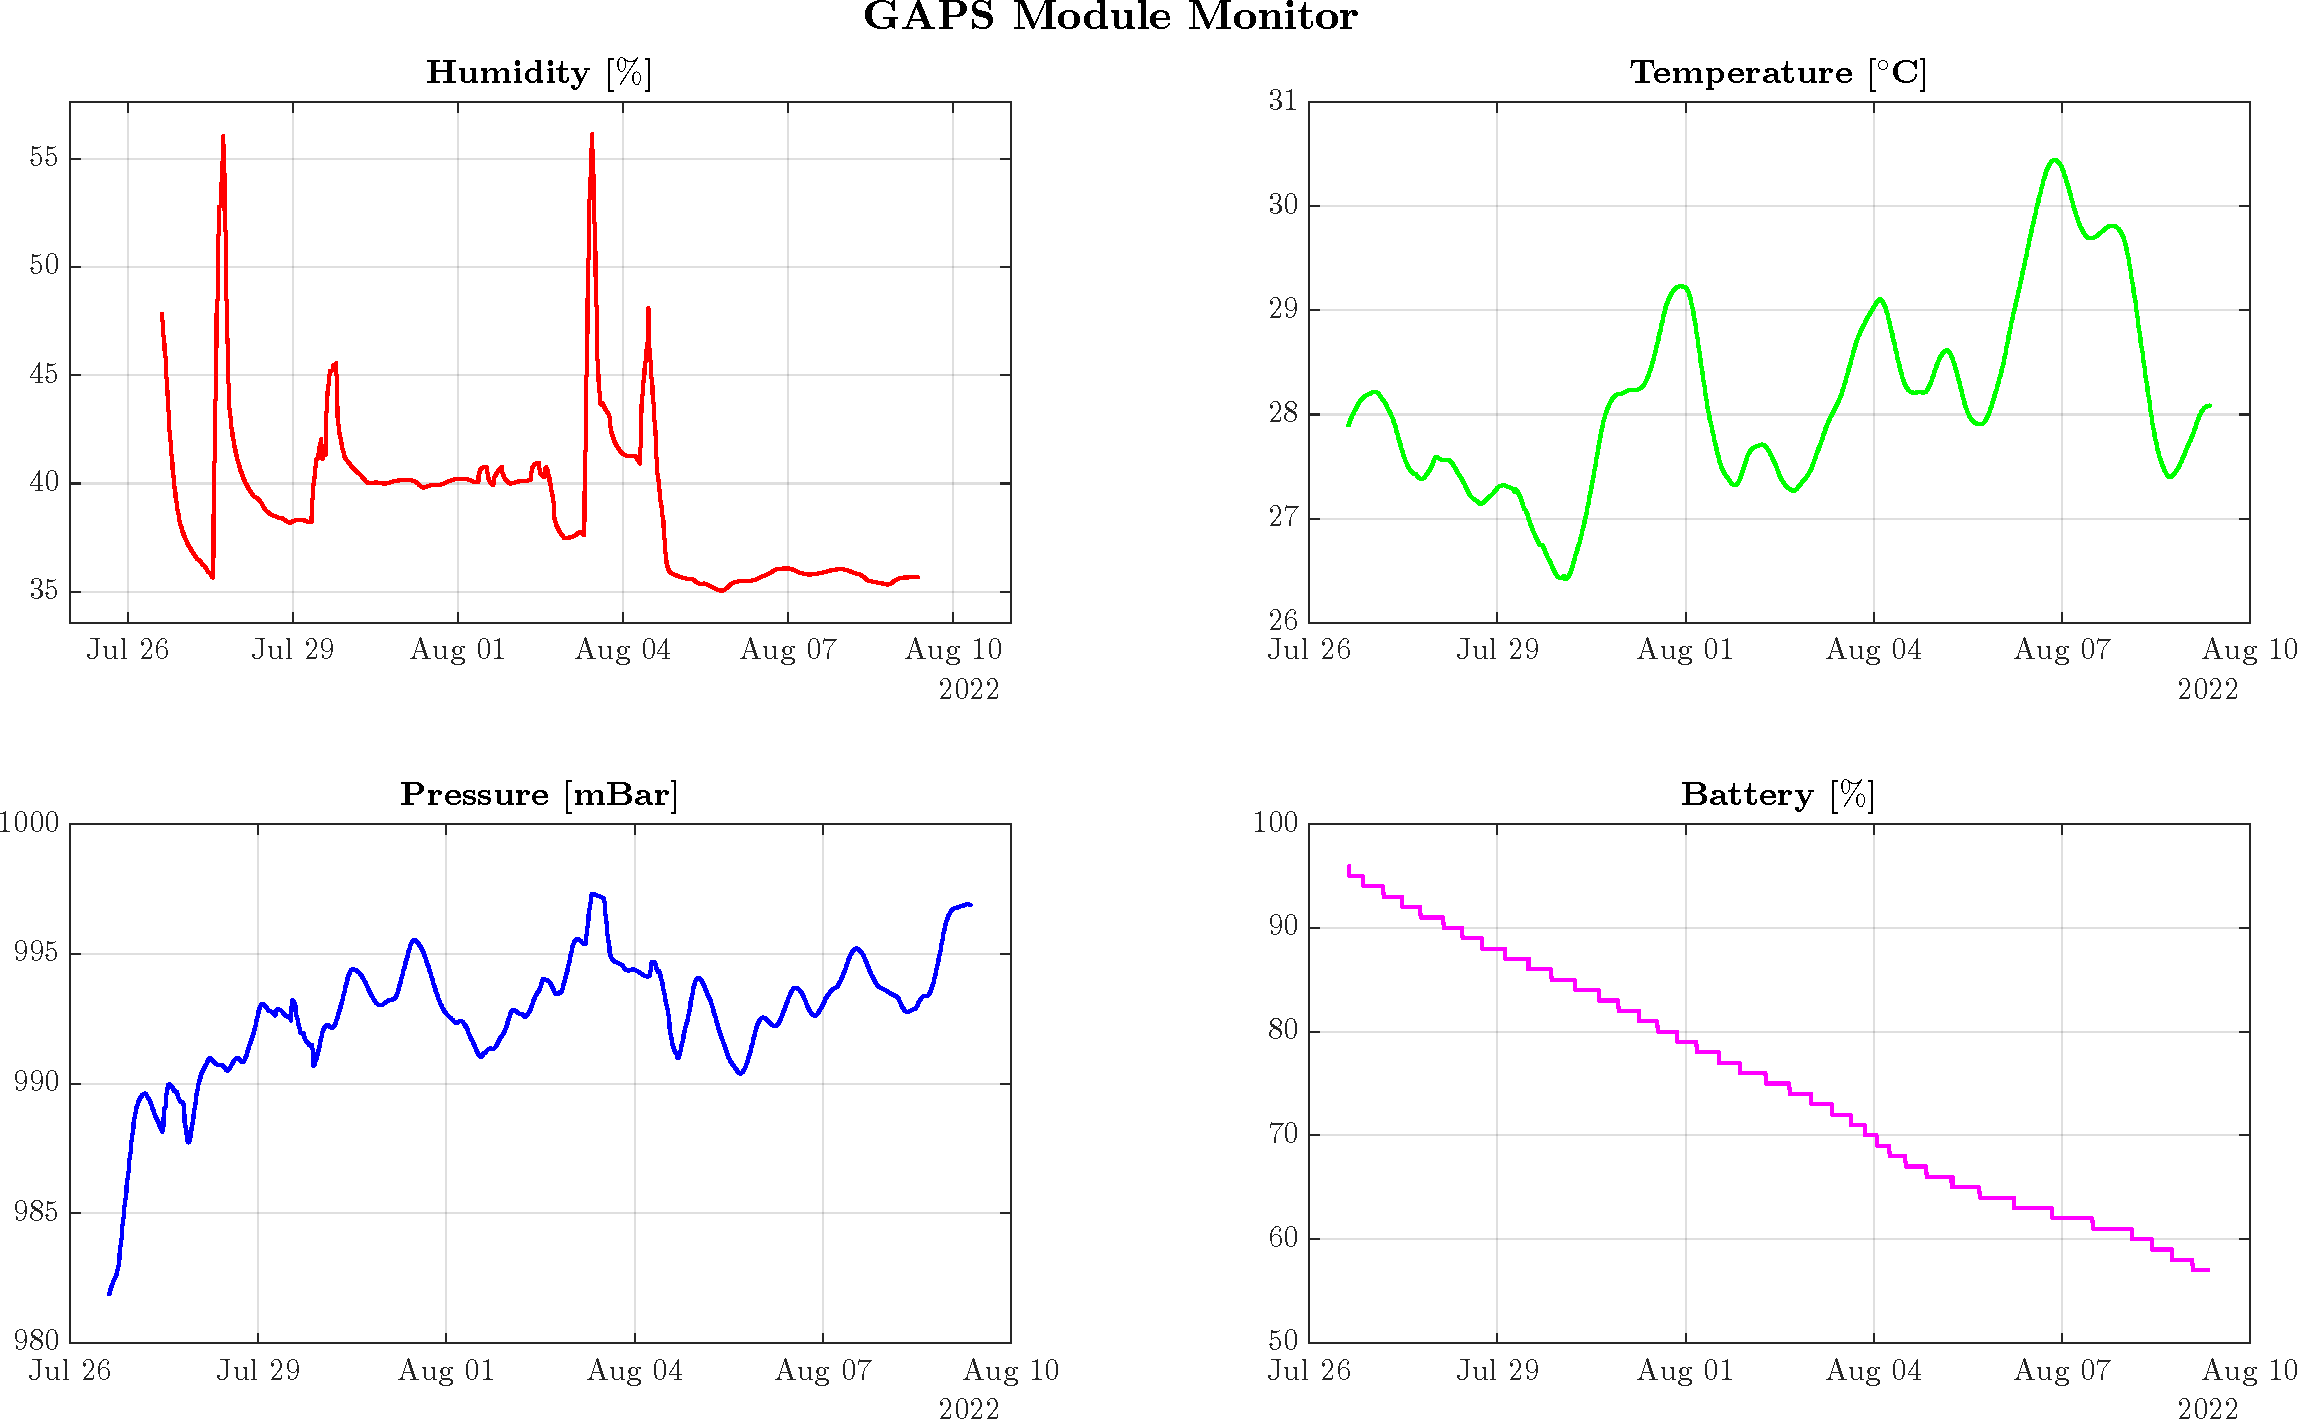
\includegraphics[width=0.7\textwidth]{Images/chap3/winter_plot.pdf} 
    \caption{GAPS Module Monitor dashboard.}
    \label{figWinterMATLABmonitor}
\end{figure}

\par
For this application, the Winter platform was programmed to transmit data every 15 minutes in a one minute-long stream in order to achieve the lowest possible energy consumption, while maintaining a sufficiently representative statistic of the internal state of the box. In fact, the device is kept in a \textit{sleep} state for the entire time interval during the course of which no data is transmitted, and all peripherals on board the platform are kept switched off. In this state, the \texttt{STM32L475R} microcontroller that the device is equipped with is in a low power consumption mode called "stop mode 2" and counts the elapsed time through the Real-Time Clock (RTC) module. Once the 15-minute count is reached, the latter is used as an interrupt to bring the platform back from the sleep state to the \textit{idle} state. In this state, the device was programmed to transmit environmental data for 1 minute, then return to the sleep state. The complete firmware code can be found on GitHub at the following \href{https://github.com/lucaghislo/winterGAPS/tree/main}{\underline{link}}.

\par
In addition to humidity data, temperature, pressure and battery level values were also acquired. The latter parameter is of fundamental importance to check the state of the battery and determine in advance when to replace it for recharging, while the humidity data was used to check the status of the desiccant bags, thus allowing to know when to replace them in order to guarantee a constant humidity level as low as possible. The data acquired by the Winter platform via the Raspberry Pi device is finally sent to a PC, on which it is plotted, as shown in \hyperref[figWinterMATLABmonitor]{Figure \ref{figWinterMATLABmonitor}}.

\begin{figure}[h!]
    \centering
    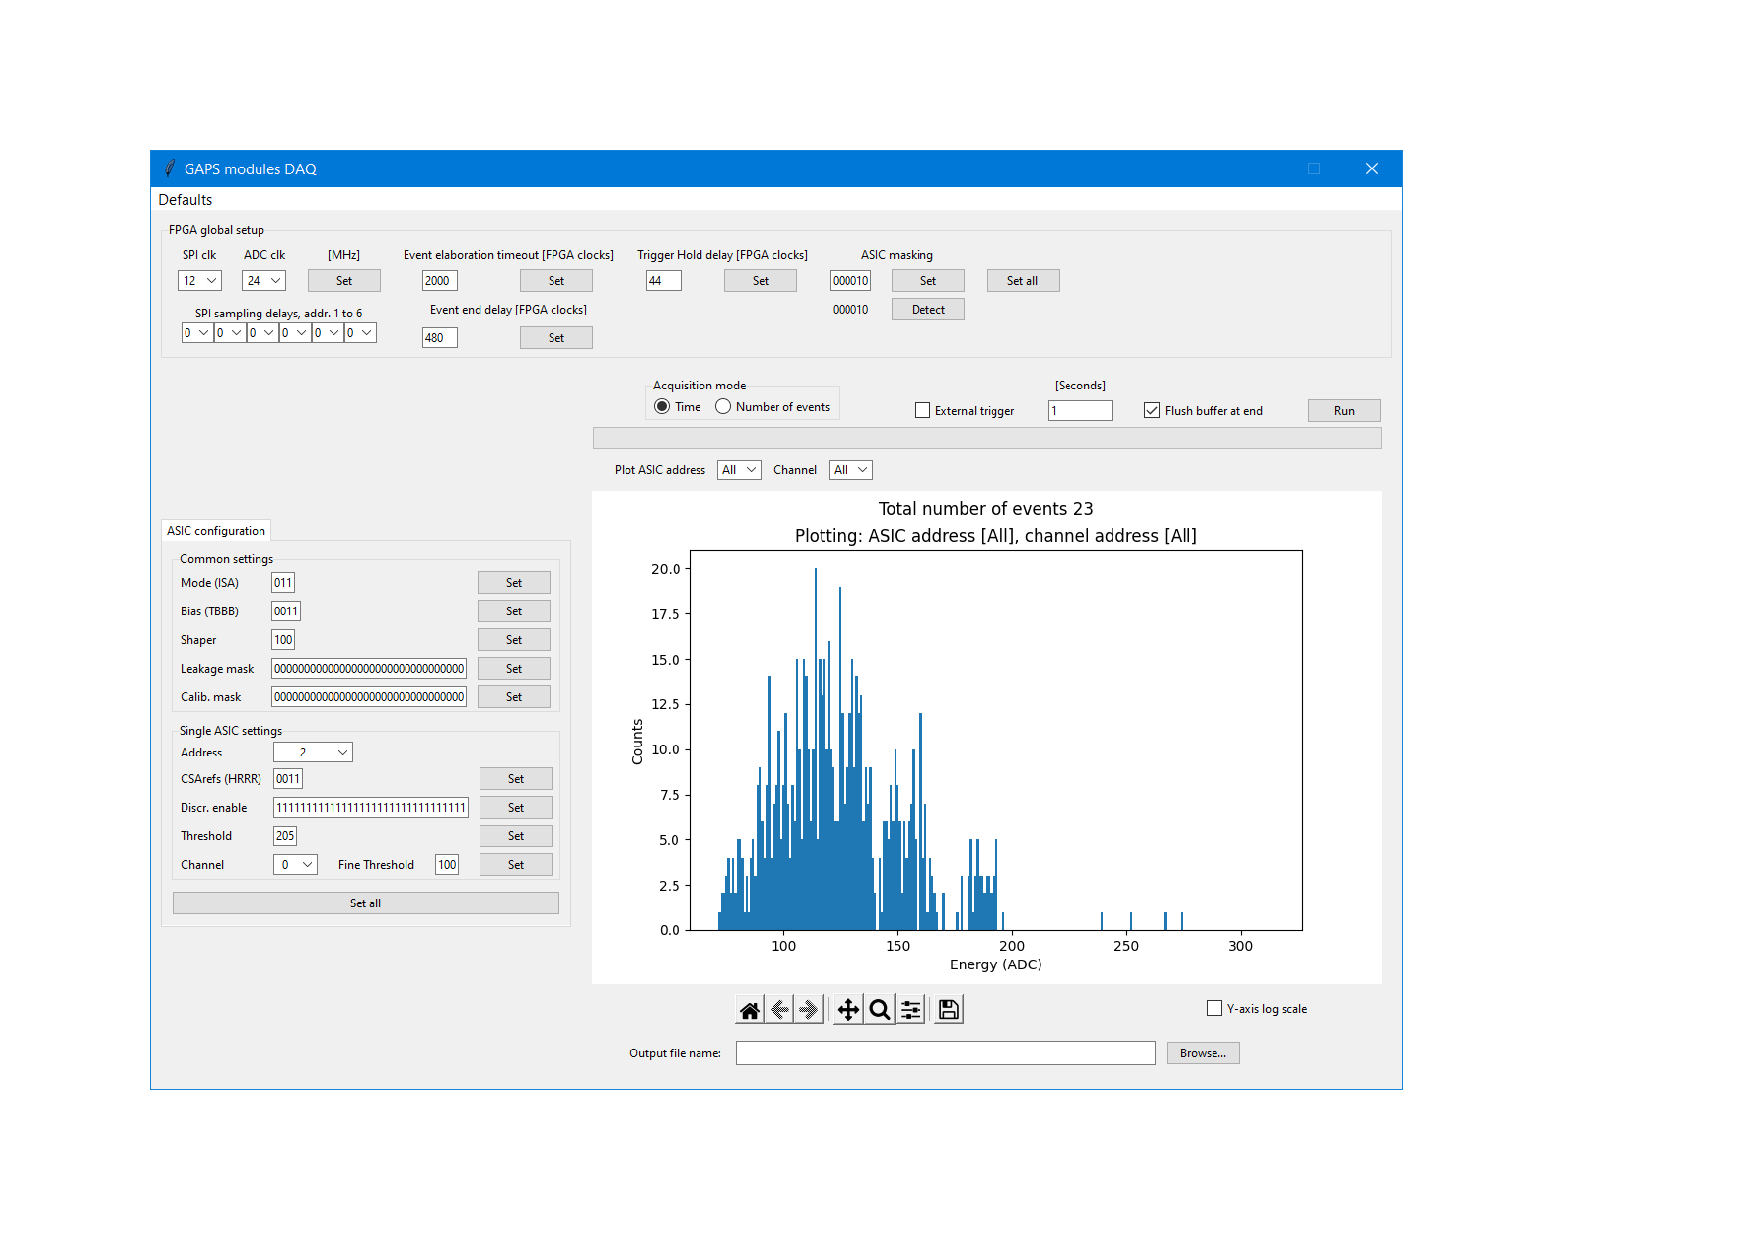
\includegraphics[width=0.7\textwidth]{Images/chap3/GAPS_DAQ.pdf}
    \caption{\texttt{GAPS\_DAQ} Python software GUI used to perform data acquisition from the Si(Li) tracker module.}
    \label{figGapsDAQpy}
\end{figure}

\par
Data acquisition from the readout electronics of the Si(Li) tracker module was performed via the \texttt{GAPS\_DAQ} version 3 application, whose main graphical user interface is shown in \hyperref[figGapsDAQpy]{Figure \ref{figGapsDAQpy}}. The software also allows the setting of the electronics and FPGA parameters, summarised in \hyperref[tabMuonASICconfig]{Table \ref{tabMuonASICconfig}}, which were varied for specific data acquisition sessions and subsequently reported, the results of which are shown in \hyperref[secMuonDetectionResults]{Section \ref{secMuonDetectionResults}}.

\begin{table}[h!]
    \centering
    \begin{tabular}{l l l} 
         \Xhline{2\arrayrulewidth}
         Parameter & Value & Description \T\B \\
         \hline
         \multirow{3}{*}{Mode (\texttt{ISA})} & \texttt{010} & Self trigger mode with Zero Suppression \T\B \\ & \texttt{011} & Self trigger mode without Zero Suppression \T\B \\ & \texttt{001} & External trigger mode without Zero Suppression \T\B \\
         Bias (\texttt{TBBB}) & \texttt{0110} & Gloabal bias regulation \T\B \\ 
         CSArefs (\texttt{HRRR}) & \texttt{0011} & \texttt{H} set to \texttt{0}, test performed at \SI{-40}{\celsius} \T\B \\ 
         Shaper & \texttt{100} & Peaking time \#4 ($\tau_{p} = \SI{0.98}{\micro\second}$) \T\B \\ 
         \Xhline{2\arrayrulewidth}
    \end{tabular}
    \caption{Main \texttt{GAPS\_DAQ} parameters settings used during data acquisition. Other parameters were kept at their default value, provided by the application.}
    \label{tabMuonASICconfig}
\end{table}


%-------------------------------------------------------------------------------
%   Experimental results
%-------------------------------------------------------------------------------

\section{Experimental results}
This Section presents the experimental results obtained during the readout electronics test, reported in \hyperref[secResultsMuonASIC]{Section \ref{secResultsMuonASIC}}, and subsequently during the cosmic muon detection experiment, the results of which are reported in \hyperref[secMuonDetectionResults]{Section \ref{secMuonDetectionResults}}.

% caratterizzazione modulo
\subsection{Module characterisation}
\label{secResultsMuonASIC}

In this Section, the tests performed on the readout electronics of the Si(Li) tracker module using the \textit{Automated test} of the \texttt{GAPS\_ModuleTester} software are presented. The purpose of these measurements, which were carried out prior to the muon detection experiment, is to verify the correct functioning of the readout electronics installed inside the assembled module equipped with Si(Li) detectors and it represents the last step in the process of testing the Si(Li) tracker readout electronics illustrated in this thesis work. In this regard, \hyperref[ch1]{Chapter \ref{ch1}} proposes the results of tests carried out on the SLIDER32 ASIC alone at different temperature steps. Consequently, \hyperref[ch2]{Chapter \ref{ch2}} proposes the tests carried out on the FEB without Si(Li) detectors and \hyperref[ch3]{Chapter \ref{ch3}} finally provides the results of the tests on the assembled module in the version intended for flight. All tests were carried out by keeping the module at a controlled temperature of \SI{-40}{\celsius} and \SI{10}{\percent} relative humidity. The Si(Li) detectors were biased with a voltage of \SI{-250}{\volt} and bit \texttt{H} was set to \texttt{0}.

% modulo a -40C con sensori a -250V H=0, tau6
\begin{figure}[h!]
    \centering
    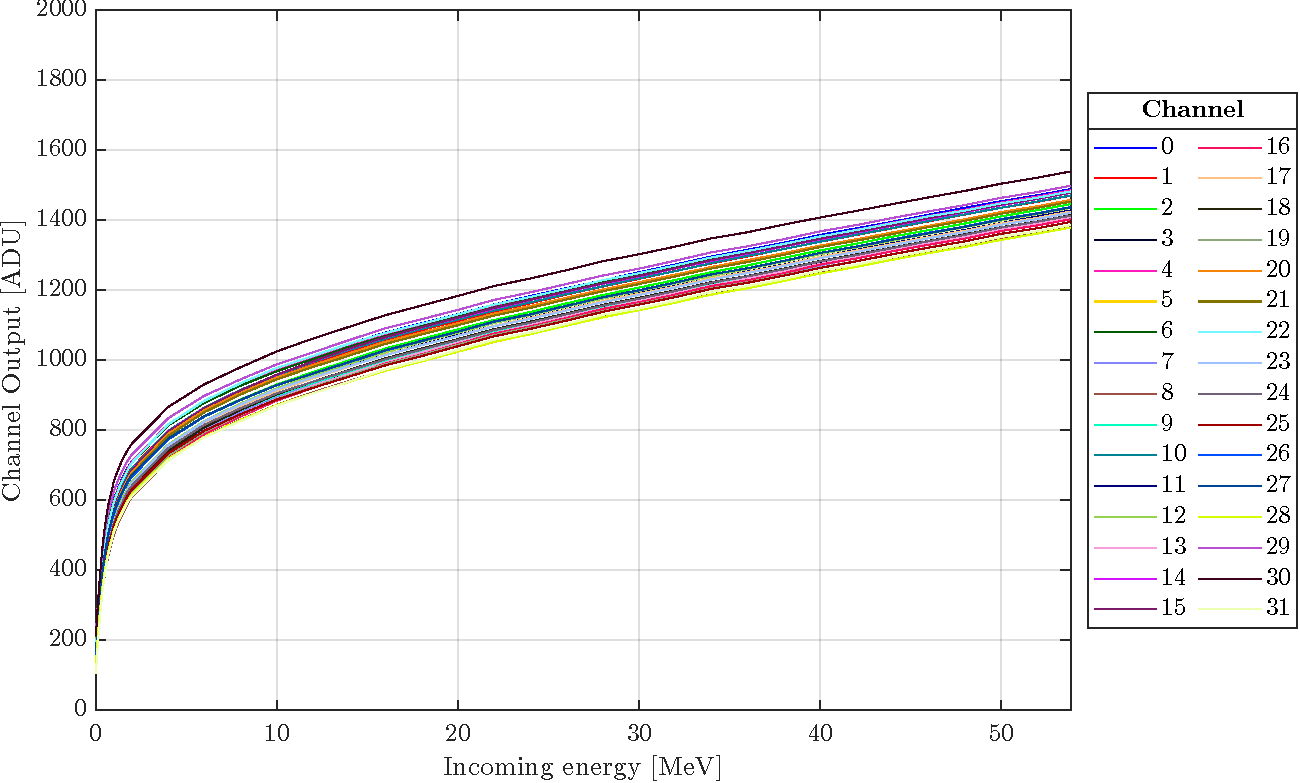
\includegraphics[width=0.65\textwidth]{Images/chap3/results/FDT_MODULE_40C_250V.pdf}
    \caption{Input-output trans-characteristics of all channels at peaking time \#6 ($\tau_{p} = \SI{1.48}{\micro\second}$) with module at \SI{-40}{\celsius}, Si(Li) detectors biased at \SI{-250}{\volt} and bit \texttt{H} set to \texttt{0}.}
    \label{figFDTmodule40C250V}
\end{figure}


\par
\hyperref[figFDTmodule40C250V]{Figure \ref{figFDTmodule40C250V}} shows the input-output trans-characteristics of all channels at peak time \#6 ($\tau_{p} = \SI{1.48}{\micro\second}$). It can be seen that all channels respond correctly and follow the desired trend defined by the dynamic signal compression feature already illustrated in \hyperref[testboardFDT]{Section \ref{testboardFDT}}.

% modulo a -40C con sensori a -250V tutti i PT H=0
\begin{figure}[h!]
    \centering
    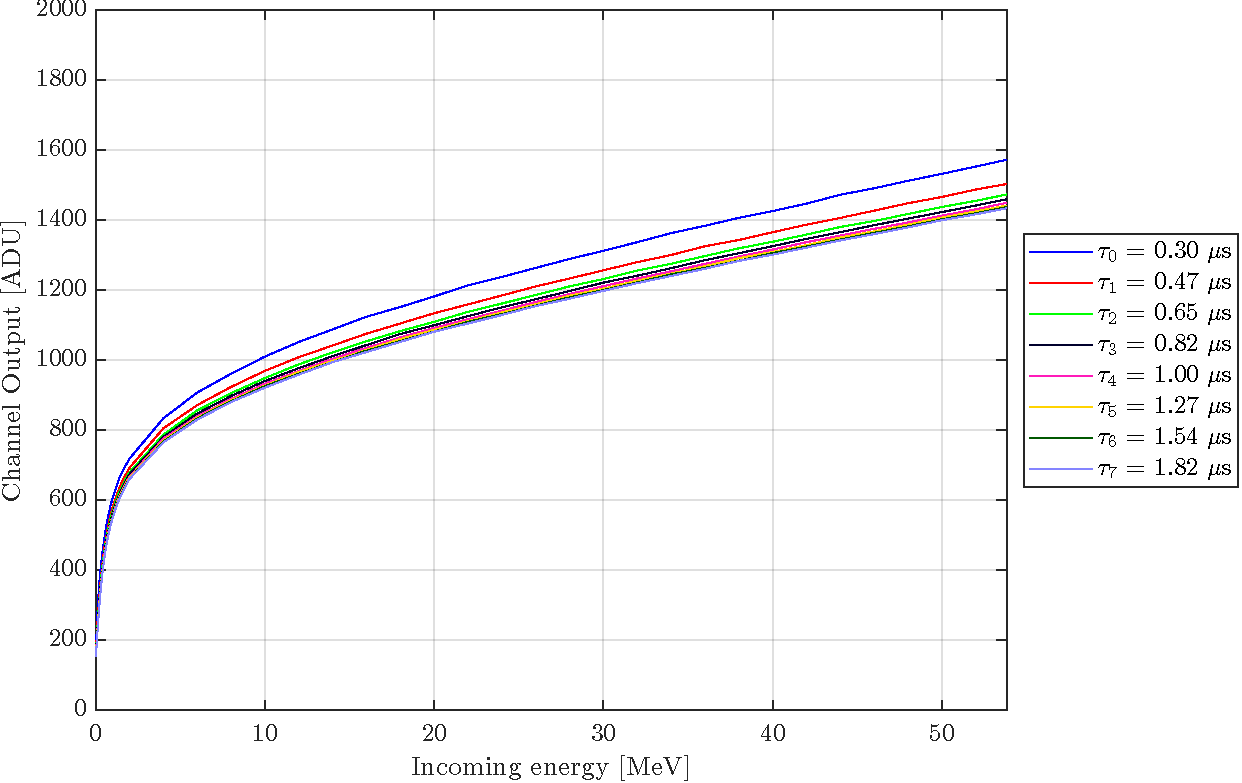
\includegraphics[width=0.65\textwidth]{Images/chap3/results/FDT_MODULE_40C_250V_allpt.pdf}
    \caption{Mean input-output trans-characteristics of all channels at all the selectable
peaking times with module at \SI{-40}{\celsius}, Si(Li) detectors biased at \SI{-250}{\volt} and bit \texttt{H} set to \texttt{0}.}
    \label{figFDTmodule40C250VALLPT}
\end{figure}

\par
\hyperref[figFDTmodule40C250VALLPT]{Figure \ref{figFDTmodule40C250VALLPT}} shows the average input-output trans-characteristics calculated over all 32 channels for each of the 8 selectable peaking times. Also in this case, the trend of the transfer function is comparable to the desired one.

% modulo a -40C con sensori a -250V tutti i PT H=0
\begin{figure}[h!]
    \centering
    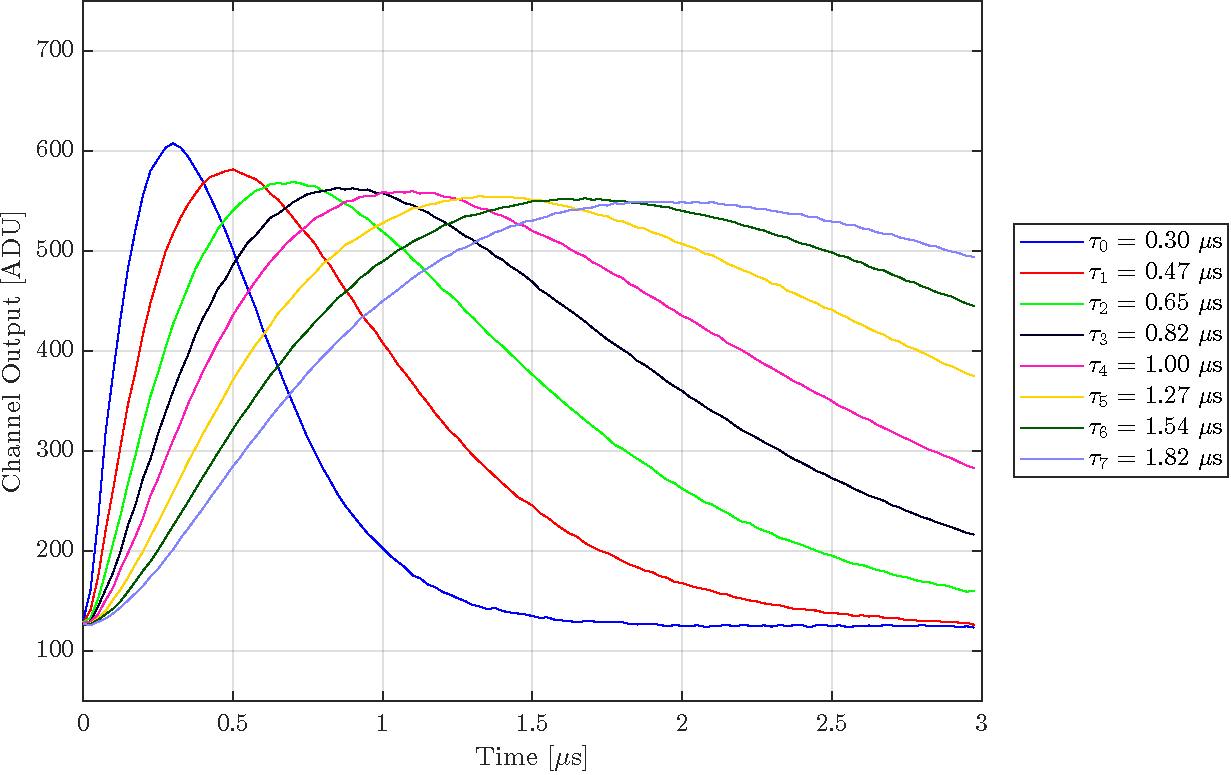
\includegraphics[width=0.65\textwidth]{Images/chap3/results/WAVEFORM_MODULE_40C_250V_allpt.pdf}
    \caption{Measured time response of the time-invariant filter for an emulated input particle energy of \SI{841}{\kilo\electronvolt} and for the 8 selectable peaking times with module at \SI{-40}{\celsius}, Si(Li) detectors biased at \SI{-250}{\volt} and bit \texttt{H} set to \texttt{0}.}
    \label{figWAVEmoduleALLPT}
\end{figure}

\par
\hyperref[figWAVEmoduleALLPT]{Figure \ref{figWAVEmoduleALLPT}} shows the measured time response of the time-invariant filter for an emulated input particle energy of \SI{841}{\kilo\electronvolt}. The response was derived for all 8 selectable peaking times. Again, the response of the shaper filter is consistent with the simulations and with the measurements carried out first on the ASIC alone via test board, illustrated in \hyperref[ch1]{Chapter \ref{ch1}}, and then on the FEB tested in \hyperref[ch2]{Chapter \ref{ch2}}.

\par
\hyperref[figENCmodule]{Figure \ref{figENCmodule}} shows the ENC graph evaluated for all 32 channels at each of the 8 selectable peaking times. From the measurements made on the ASIC alone and illustrated in \hyperref[figENCwomean]{Figure \ref{figENCwomean}} (on the right), it can be seen that the 8 channels on which an equivalent number of \SI{40}{\pico\farad} capacitors were mounted to simulate the detector strips, demonstrate a lower ENC value than that measured on the assembled module. This could be related to the measurement setup, which for the tests on the ASIC involved the use of a metal box to shield electromagnetic interference present in the test environment. In contrast, the module was tested by placing it in the climatic chamber without any shielding, as it will be during flight.

\begin{figure}[h!]
    \centering
    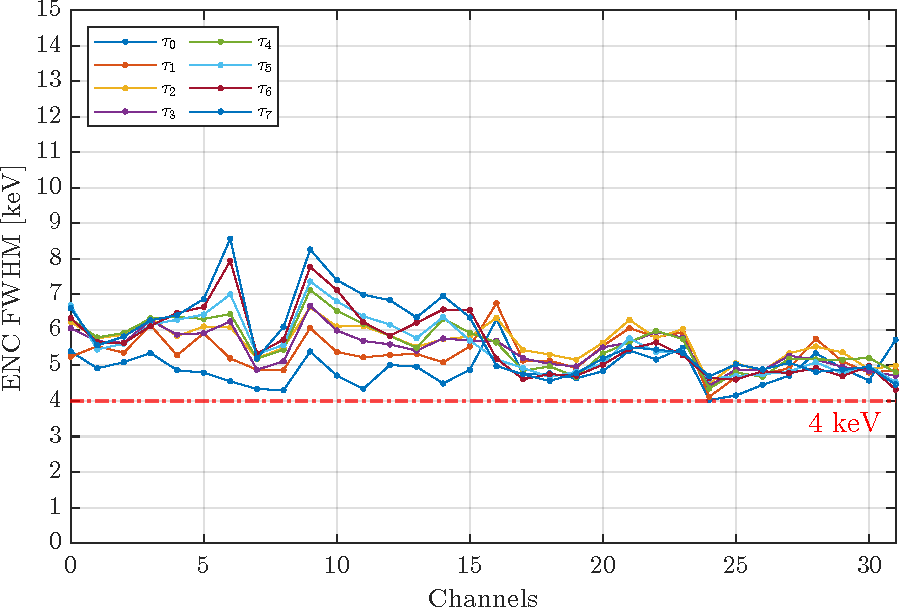
\includegraphics[width=0.63\textwidth]{Images/chap3/results/ENC_MODULE_40C_250V.pdf}
    \caption{ENC without external interference evaluated with module at \SI{-40}{\celsius}, Si(Li) detectors biased at \SI{-250}{\volt} and bit \texttt{H} set to \texttt{0}.}
    \label{figENCmodule}
\end{figure}

% leakage current
The leakage current associated with Si(Li) detectors was also evaluated. The measurement was carried out at a constant temperature of \SI{-40}{\celsius} using the \textit{manual test} provided by the \texttt{GAPS\_ModuleTester} software already presented in \hyperref[sec21]{Section \ref{sec21}}. The software outputs a text file containing 1000 acquisitions of the leakage current value reported in ADU, as obtained at the output of the ADC located in the portion of the circuit dedicated to both temperature and leakage current measurements. In order to activate the latter mode of operation, bit \texttt{I} of the \texttt{ISA} triplet must be set to \texttt{1}. The conversion from ADU to Ampere is carried out by means of the following formula, which takes into account the design parameters associated with the circuit used to measure the leakage current:

\begin{equation}
    I_{leakage} = \frac{(1024 - ADC_{code}) \cdot \SI{1.72}{\milli\volt}}{3.87 \cdot 10 \cdot R}
\end{equation}

\noindent
where $ADC_{code}$ is comprised between 0 and 2047 ADU, \SI{1.76}{\milli\volt} represents the ADC \textit{Least Significant Bit} (LSB), $3.87$ is the gain of the S\&H, $10$ is the gain of the current mirror implemented in the measuring circuit and $R$ equals to $\SI{223.7}{\kilo\ohm}$. The latter parameter represents the value of the resistor employed for the conversion from current to voltage that is then sampled by the S\&H and later digitised by the ADC.

\begin{figure}[h!]
    \centering
    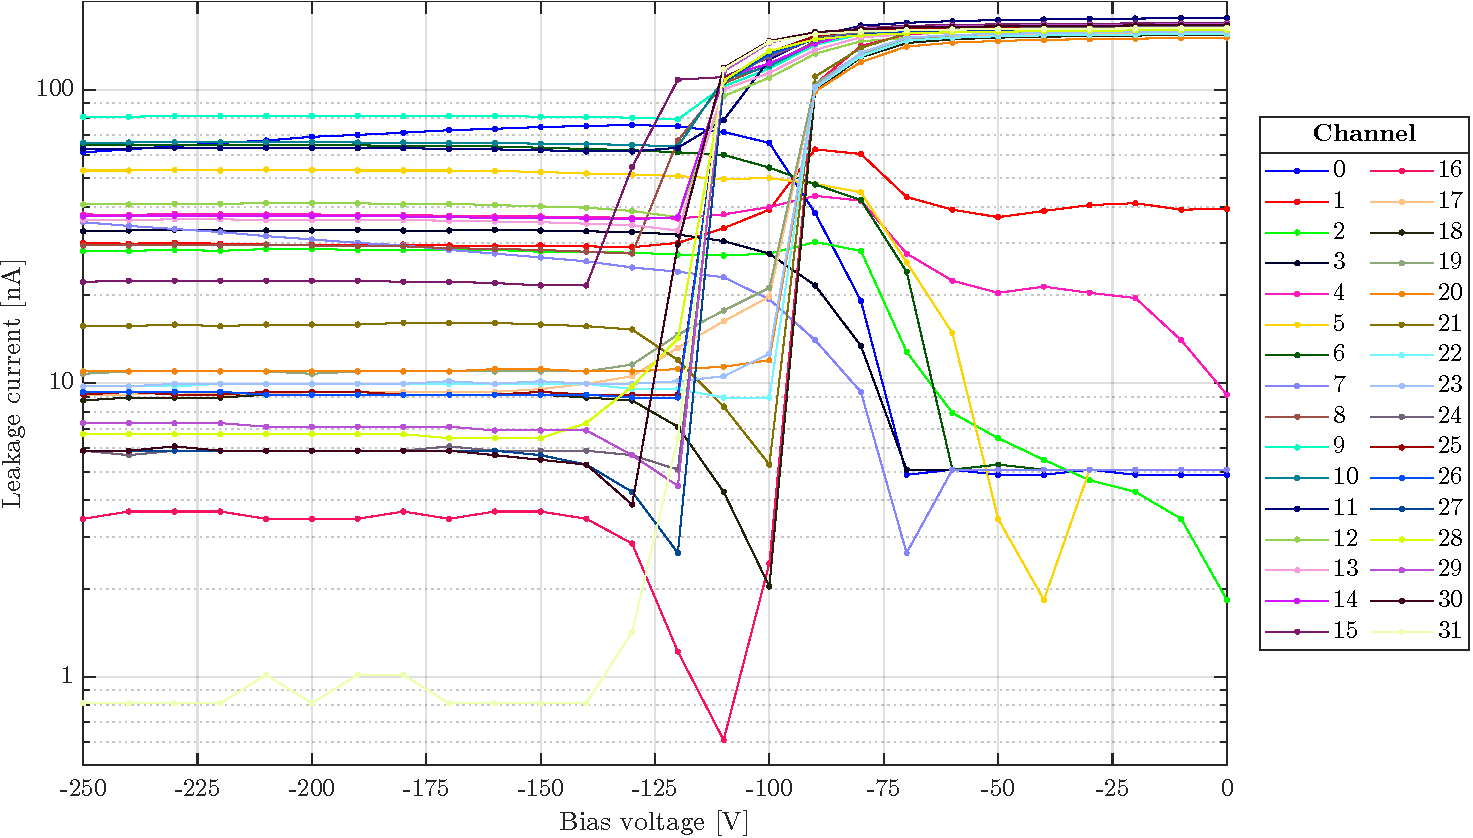
\includegraphics[width=0.8\textwidth]{Images/chap3/results/leakage_current.pdf}
    \caption{Si(Li) detectors leakage current measured for all 32 channels at a constant temperature of \SI{-40}{\celsius} for detector biasing voltage comprised between \SI{0}{\volt} and \SI{-250}{\volt}.}
    \label{figLeakageVoltages}
\end{figure}

From the graph in \hyperref[figLeakageVoltages]{Figure \ref{figLeakageVoltages}}, it can be seen that the leakage current decreases for most channels as the nominal value of the detector bias voltage set at \SI{-250}{\volt} is reached. 

\par
In order to better study the leakage current value of each of the 32 channels at the operating voltage of \SI{-250}{\volt}, the graph in \hyperref[figLeakage250V]{Figure \ref{figLeakage250V}} shows its trend as a function of channel. It can be seen that the first 16 channels (between 0 and 15) take on average 10 times more leakage current than the last 16 channels (between 16 and 31). In these channels, the highest leakage current value per individual channel is also measured, amounting to \SI{71.13}{\nano\ampere} for channel 9. In contrast, the lowest leakage current value was measured in channel 31 and evaluated at \SI{1.59}{\nano\ampere}.

\begin{figure}[h!]
    \centering
    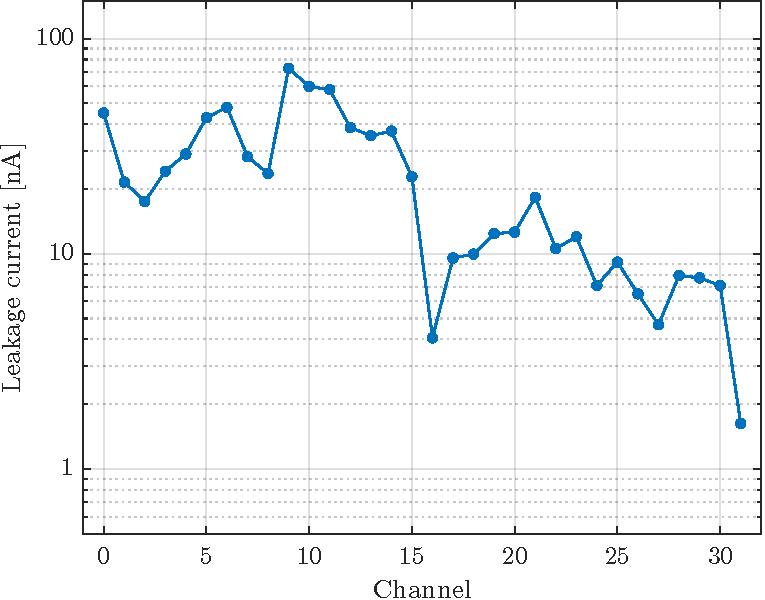
\includegraphics[width=0.6\textwidth]{Images/chap3/results/leakage_current_ch_250V.pdf}
    \caption{Si(Li) detectors leakage current measured for all 32 channels at a constant temperature of \SI{-40}{\celsius} for detector biasing voltage fixed to \SI{-250}{\volt}.}
    \label{figLeakage250V}
\end{figure}

\par
This behaviour can be explained by taking into account the fact that each of the detectors mounted within the Si(Li) tracker module under investigation has its own peculiar characteristics that can induce quite natural variations in the leakage current value. Overall, the total leakage current on all 32 channels was evaluated at \SI{746.11}{\nano\ampere} and is comparable to the value read directly from the high voltage power supply used during the test.

% ESPERIMENTO RILEVAZIONE AMERICIO
\par
As a final procedure for characterising the module, an experiment was carried out using a sample of Americium 241, commonly referred to as \ce{^{241}Am}.  The latter is a man-made radioactive isotope with a half-life of 432.2 years and is usually found in smoke detectors. The source is an alpha emitter, and in the decay process it also kicks out gamma radiation at \SI{59.54}{\kilo\electronvolt} and \SI{26.34}{\kilo\electronvolt} \cite{agencyfortoxicsubstancesanddiseaseregistry_2004_chemical}. A sample of Americium 241 was placed below Si(Li) detector \#0 (channels 0 to 7) and in order to determine the best threshold level to be set on these channels with the aim of detecting at least the \SI{59.54}{\kilo\electronvolt} peak, a charge scan was first performed and it is presented in \hyperref[figChargeScan]{Figure \ref{figChargeScan}} on the left. 

\par
During this test, the threshold value is kept constant and the value of the injected charge is varied in order to determine the channel's trigger profile, expressed in trigger probability from \SI{0}{\percent} to \SI{100}{\percent}. This test was performed using the \textit{manual test} of the \texttt{GAPS\_ModuleTester} software already described in \hyperref[sec21]{Section \ref{sec21}}, in which the injected charge range and step can be specified. For this specific test, the range was set from a minimum of \SI{0}{DAC_{units}} to a maximum of \SI{300}{DAC_{units}} with steps of \SI{1}{DAC_{units}}. Repeated tests led to the selection of a threshold value of \texttt{214}, whose equivalent energy value can be seen in \hyperref[figChargeScan]{Figure \ref{figChargeScan}} (on the right) for channels 0 to 7 and is equivalent to \SI{22.65}{\kilo\electronvolt} on average. On the same graph, the ENC trend evaluated on the corresponding channels is shown in blue. 

\begin{figure}[h!] % 0.505 % 0.44
    \centering
    \begin{tabular}{cc}
        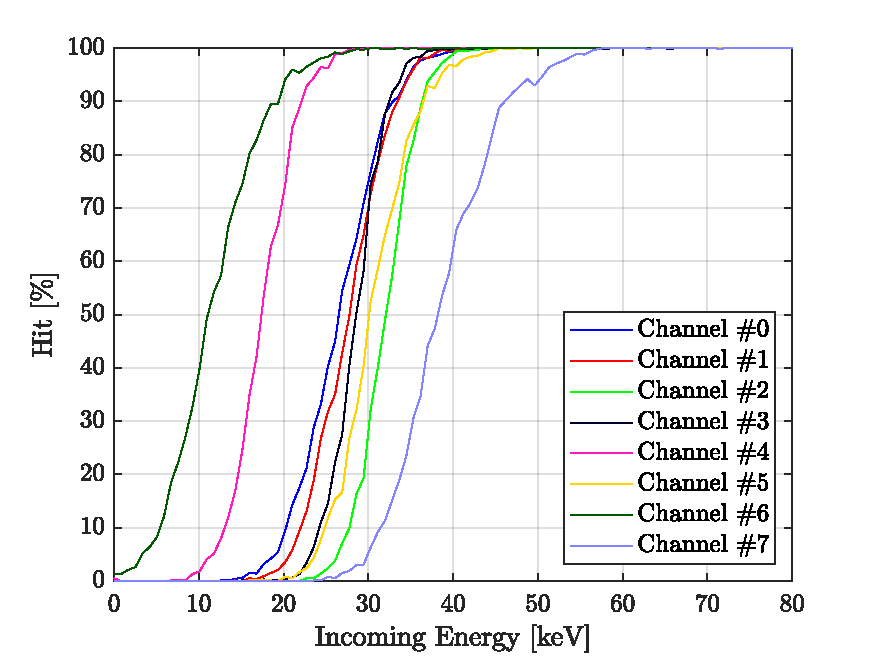
\includegraphics[width=0.505\textwidth]{Images/chap3/results/americio/Threshold Scan - Detector 0 - TH214.pdf} & 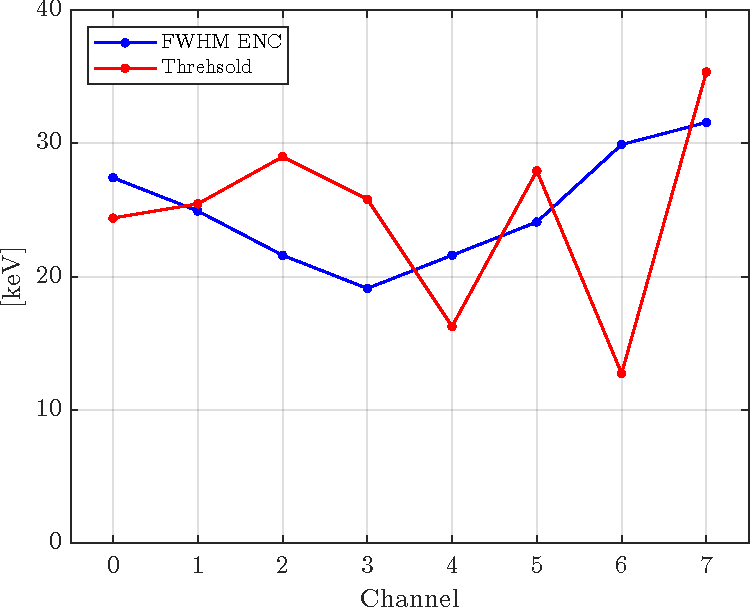
\includegraphics[width=0.44\textwidth]{Images/chap3/results/americio/ENC_channels.pdf}\\
    \end{tabular}
    \caption{Charge scan performed on channels 0 to 7 of detector \#0 (on the left) with corresponding ENC and threshold values (on the right).}
    \label{figChargeScan}
\end{figure}

\par
Both of the previously mentioned parameters were obtained from the charge scan by interpolating the Cumulative Distribution Function (CDF) of the normal distribution reported in \hyperref[eqCDFnormale]{Equation \ref{eqCDFnormale}}. The mean value ($\mu$) equals to the threshold associated to each channel and corresponds to the charge value that causes the channel to trigger in \SI{50}{\percent} of the cases. On the other hand, the FWHM ENC value was obtained by multiplying the corresponding standard deviation ($\sigma$) by the \textit{Fano factor}, as reported in \hyperref[ENCchargeScan]{Equation \ref{ENCchargeScan}}. \\

\begin{equation}
    F(x) = \Phi \left(\frac{x-\mu}{\sigma}\right) = \frac{1}{2} \left[ 1 + erf \left( \frac{x-\mu}{\sigma \sqrt{2}} \right) \right]
    \label{eqCDFnormale}
\end{equation}

\vspace{0.15cm}

\begin{equation}
    ENC = \sigma \cdot 2.35
    \label{ENCchargeScan}
\end{equation}

\par
The acquisition was carried out for a duration of 1 hour in self-trigger mode with peak time no. 4 ($\tau_{p} = \SI{0.98}{\micro\second}$) and discriminator enable mask set to \texttt{0x0000FF} in order to activate only the first 8 channels (channel 0 to 7) belonging to detector \#0. As can be seen from the graph in \hyperref[figAmericioTHR214]{Figure \ref{figAmericioTHR214}}, in addition to the peak associated with the pedestal, there is first of all a peak at approximately \SI{59}{\kilo\electronvolt}. It is also possible to observe the classic \textit{Compton shoulder} (also called \textit{Compton edge}) arranged approximately between the first peak and a second one positioned at about \SI{26}{\kilo\electronvolt}. As mentioned above, both peaks can be associated with those present in the emission spectrum of Americium 241 caused by gamma decays.

\begin{figure}[h!]
    \centering
    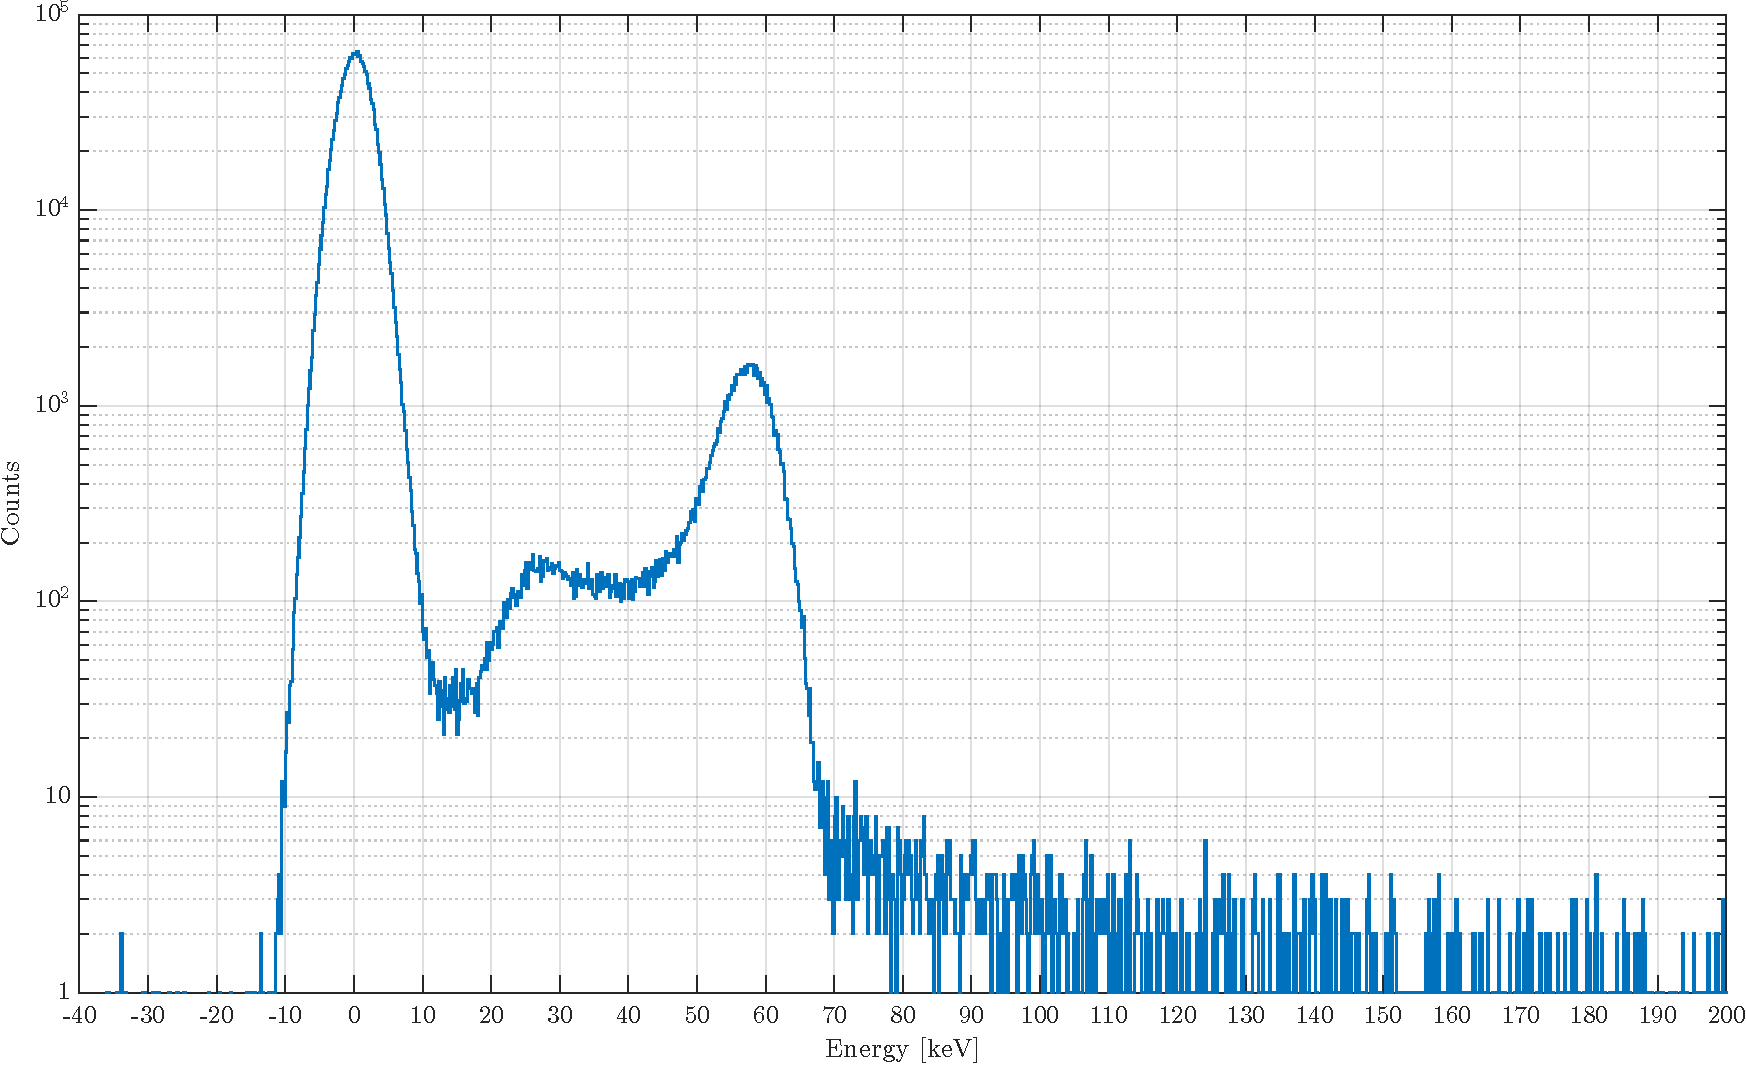
\includegraphics[width=0.8\textwidth]{Images/chap3/results/americio/ch4_americio_log.pdf}
    \caption{Self trigger acquisition carried out using the \ce{^{241}Am} sample with global threshold set to \texttt{214} and channels 0 to 7 enabled (detector \#0).}
    \label{figAmericioTHR214}
\end{figure}

\par
As highlighted by the estimation of the threshold value associated with channels 0 to 7 (detector \#0), it is possible to show how this latter parameter varies around the mean value reaching values higher than the lowest energy peak recorded around \SI{26.34}{\kilo\electronvolt}, which would ideally make it impossible to measure. The explanation for this is linked to the presence of channels firing at lower energies, such as channel 6, whose threshold is \SI{10.29}{\kilo\electronvolt}, thus making it possible to measure this second peak as well.

\begin{figure}[h!]
    \centering
    \begin{tabular}{cc}
        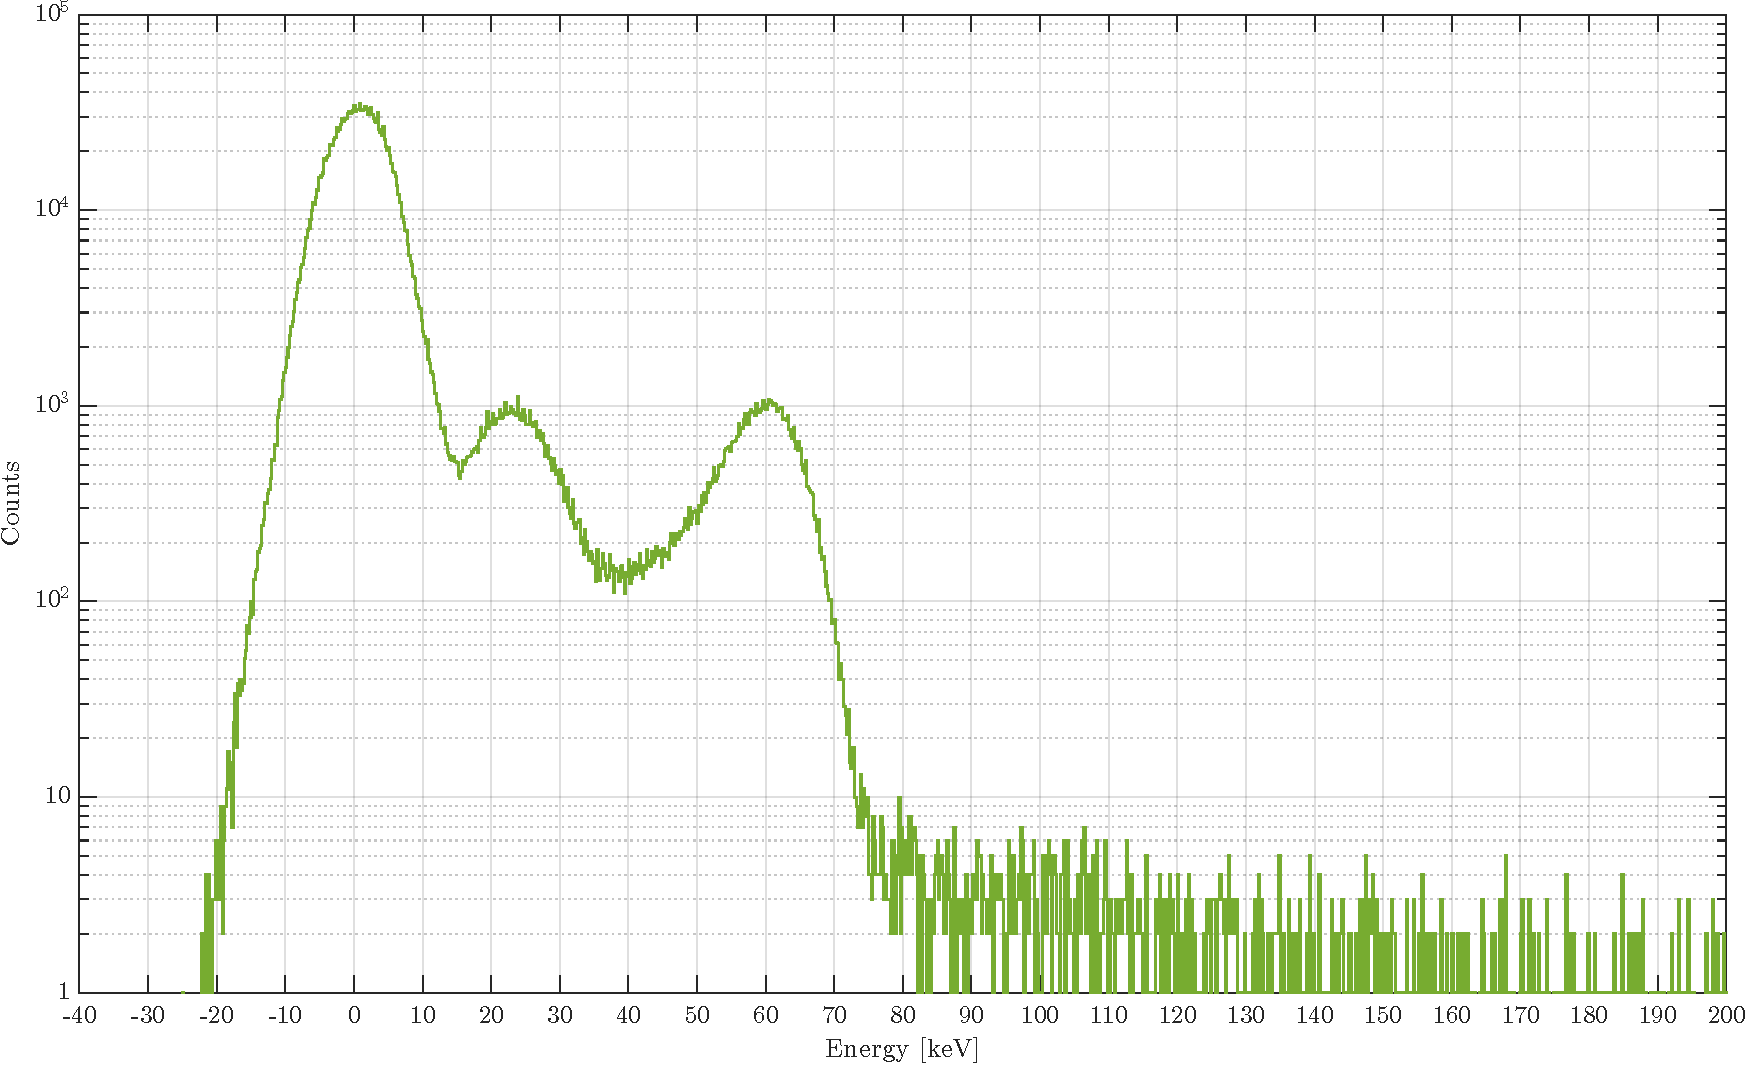
\includegraphics[width=0.47\textwidth]{Images/chap3/results/americio/ch4_americio_log_ch6.pdf} & 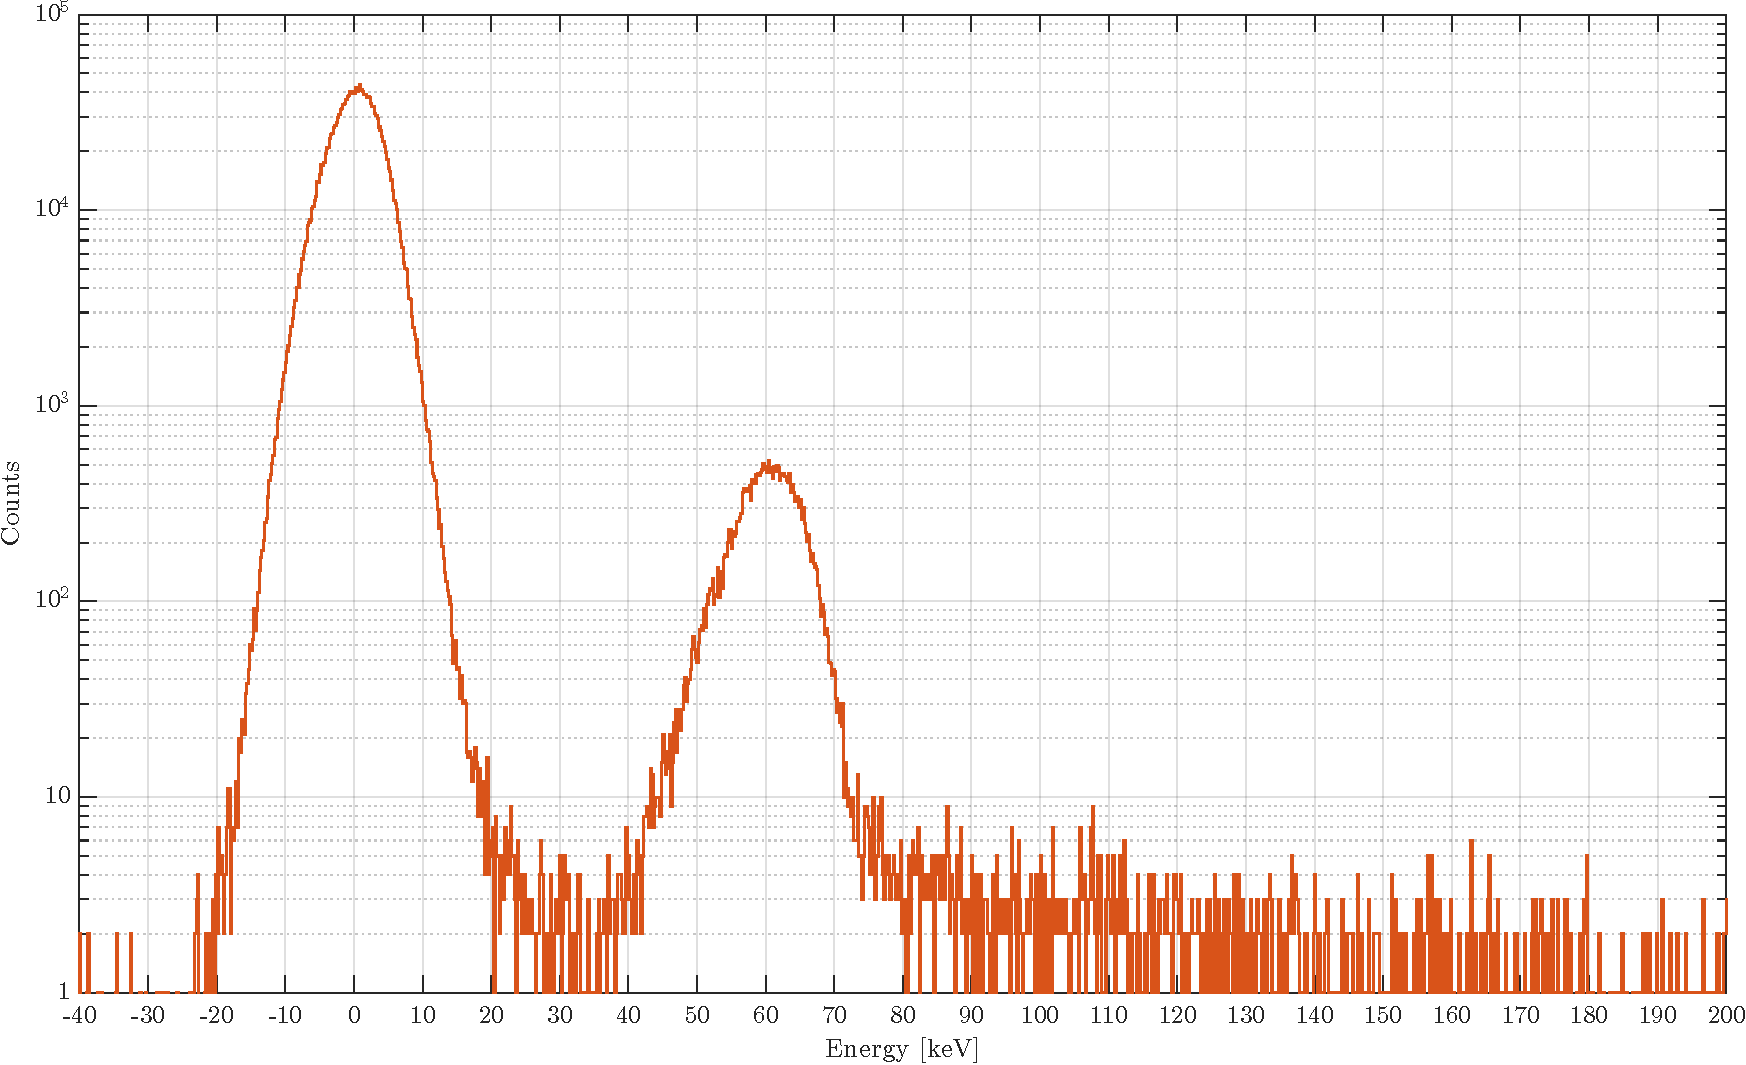
\includegraphics[width=0.47\textwidth]{Images/chap3/results/americio/ch4_americio_log_ch7.pdf}\\
    \end{tabular}
    \caption{Self trigger acquisition carried out using the \ce{^{241}Am} sample with global threshold set to \texttt{214} on channel 6 (on the left) and on channel 7 (on the right).}
    \label{figAmericioCH6-7}
\end{figure}

\par
This phenomenon can be seen in \hyperref[figAmericioCH6-7]{Figure \ref{figAmericioCH6-7}}, which shows on the left the measurement made on channel 6 alone, in which the peak at \SI{26.34}{\kilo\electronvolt} is visible. On the contrary, the energy spectrum recorded on channel 7 is presented on the left, which, having a threshold of \SI{32.98}{\kilo\electronvolt}, does not record the lowest energy peak, measuring only that at \SI{59.54}{\kilo\electronvolt}.

% rilevazione muoni
\subsection{Cosmic muon detection}
\label{secMuonDetectionResults}

This Section reports the results obtained during the muon detection experiment. Data acquisition was performed both in self-trigger mode, in which the sampling signal is generated internally starting from the information provided by the zero-crossing discriminator output signal, and in external trigger mode. In the latter mode, the trigger signal is provided by the \textit{ArduiSiPM} device, previously illustrated in \hyperref[secArduSiPM]{Section \ref{secArduSiPM}}, at the moment when an interaction event is recorded in the scintillator located below one of the sensors.

\par
\hyperref[figMUONSconfronto]{Figure \ref{figMUONSconfronto}} shows in blue the result of the acquisition performed for a duration of 1 hour in self-trigger mode with global threshold set to \texttt{100}. The plot also shows a comparison with the measurements carried out by INFN Napoli (in red) and MIT (in green). It can be seen that both the low and high energy peaks, representing noise and muons respectively, are in correspondence with those recorded by the first two measurements.

\begin{figure}[h!]
    \centering
    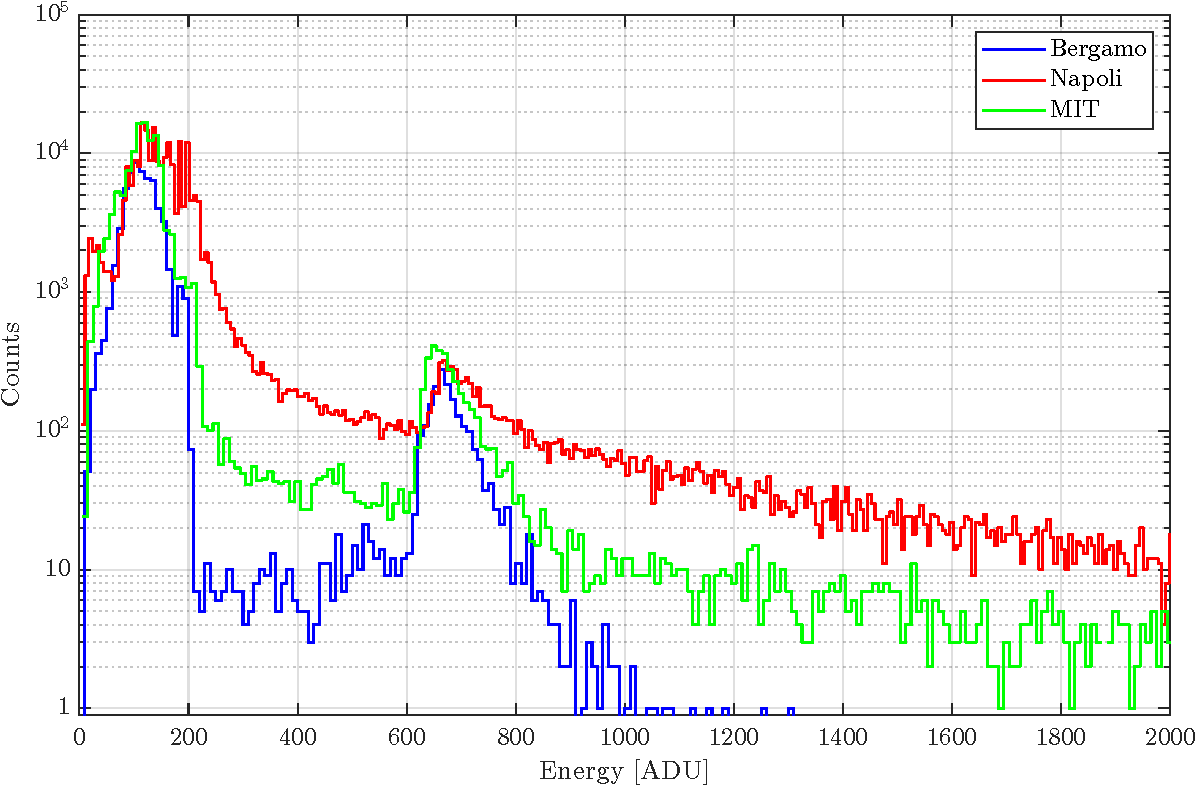
\includegraphics[width=0.75\textwidth]{Images/chap3/results/muons/incoming_energy_comparison.pdf}
    \caption{ Self trigger acquisition with global threshold set to \texttt{100} (in blue) compared to acquisitions performed by INFN Napoli (in red) and MIT (in green).}
    \label{figMUONSconfronto}
\end{figure}

% muoni self trigger threshold 130 confronto zero suppression
\begin{figure}[h!]
    \centering
    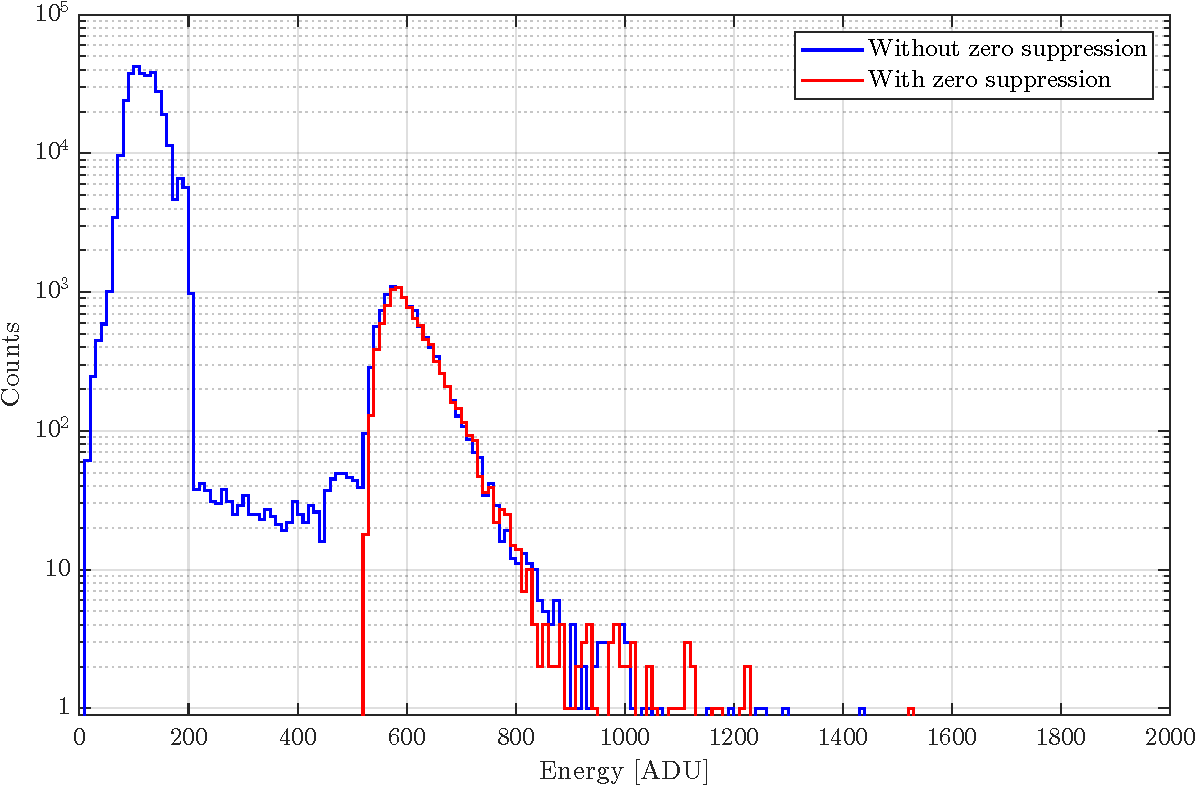
\includegraphics[width=0.75\textwidth]{Images/chap3/results/muons/incoming_energy_zero_suppr_thr130.pdf}
    \caption{Self trigger acquisition with global threshold set to \texttt{130} without zero suppression (in blue) and with zero suppression (in red).}
    \label{figMUONselfZS}
\end{figure}

\par
On the other hand, \hyperref[figMUONselfZS]{Figure \ref{figMUONselfZS}} shows the same plot illustrated above (in blue) overlaid in red with the measurement carried out under the same conditions but with the Zero Suppression (ZS) feature activated. The latter represents a channel reading mode where the output of the channel, sampled by the ADC, can be read with the dedicated read procedure only if the SOT comparator output of that channel is 1 (namely, if the shaper output is higher than the
set threshold).

\par
The same representation of the acquisition carried out in self trigger mode with zero suppression channel readout mode activated is shown in \hyperref[figMUONlandau]{Figure \ref{figMUONlandau}}, in which it is presented on a linear scale and not logarithmic as previously done. Superimposed on the same plot in green is the profile of the \textit{Landau} distribution, which almost perfectly traces the trend of the underlying data. The latter represents the distribution of energy lost by ionization of a charged particle in a thin layer of matter, that in this case is represented by the Si(Li) detector on which muons impact.

% interpolazione landau threshold 130 self trigger zero suppression
\begin{figure}[h!]
    \centering
    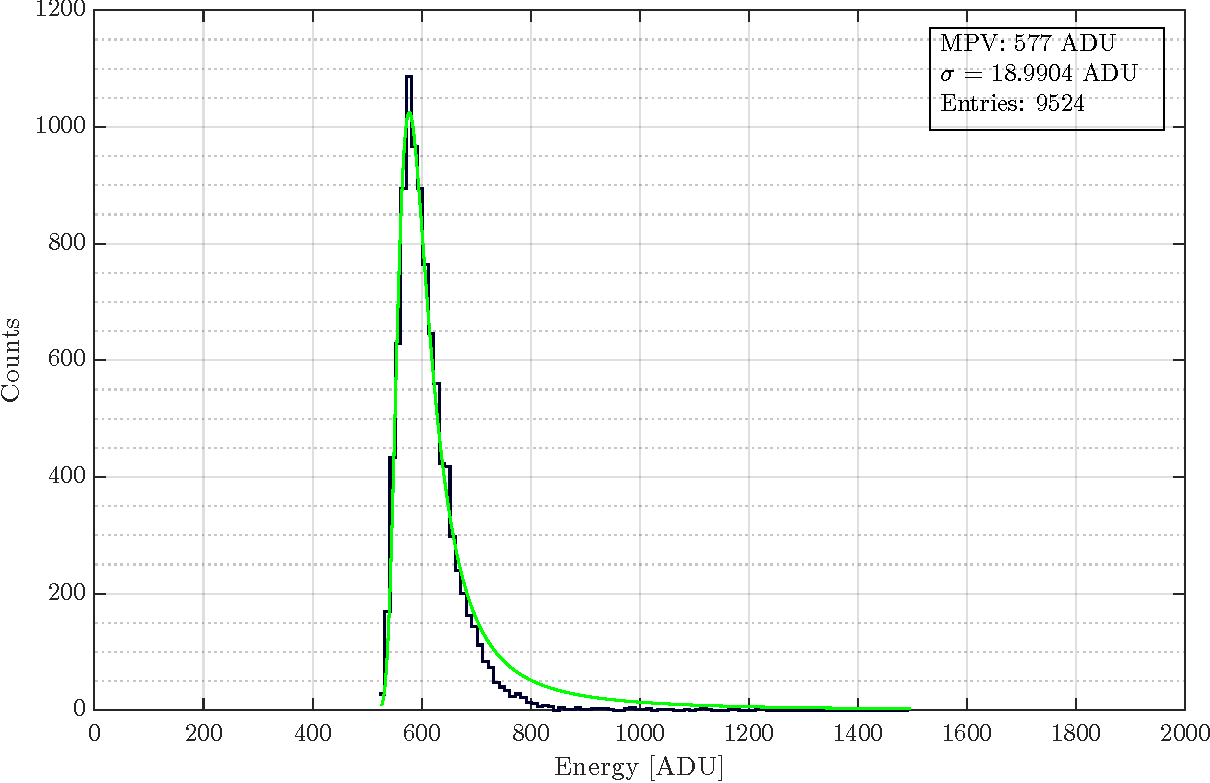
\includegraphics[width=0.75\textwidth]{Images/chap3/results/muons/incoming_energy_thr130_ZS_landau.pdf}
    \caption{Self trigger acquisition with global threshold set to \texttt{130} and zero suppression following the Landau distribution highlighted in green.}
    \label{figMUONlandau}
\end{figure}

\par
The most interesting result of the entire experiment is represented in \hyperref[figMUON4sensors]{Figure \ref{figMUON4sensors}}, which depicts the energy spectrum at the input of each of the 4 Si(Li) detectors, with detector 2 (channels 16 to 23) highlighted in red, i.e. the Si(Li) detector below which the scintillator was placed.

\par
The acquisition represented by the plot was carried out in external trigger mode and lasted 2 hours. The global threshold was set to \texttt{130} and the trigger hold delay was set to 34 FPGA clocks. The latter parameter was estimated experimentally through tests, and is described below. It can be seen that in all 4 detectors there is a low-energy peak representing noise (the pedestal), as the detection was carried out without zero suppression. The interesting result, however, can be seen in channels 16 to 23 highlighted in red. In them, a higher energy peak is visible, roughly between 400 ADU and 800 ADU, representing the energy released by cosmic muons as they pass through the Si(Li) detector strips. This behaviour serves as a proof of concept of the operating principle on which the entire GAPS experiment is based, demonstrating how a scintillator placed at a known distance from the Si(Li) detector is able to intercept cosmic muons, allowing the energy released in the Si(Li) detector to be measured by the readout electronics, as implemented in the experiment with the Time Of Flight (TOF) system, described in \hyperref[appendixGAPSexperiment]{Appendix \ref{appendixGAPSexperiment}}. A 32-channel representation of the same acquisition in which the phenomenon can be observed for each individual channel is available in \hyperref[appendix32CHmuons]{Appendix \ref{appendix32CHmuons}}.

% Plot per rimpiazzare visualizzazione a 32 canali singoli
\begin{figure}[h!]
    \centering
    \begin{tabular}{c c}
         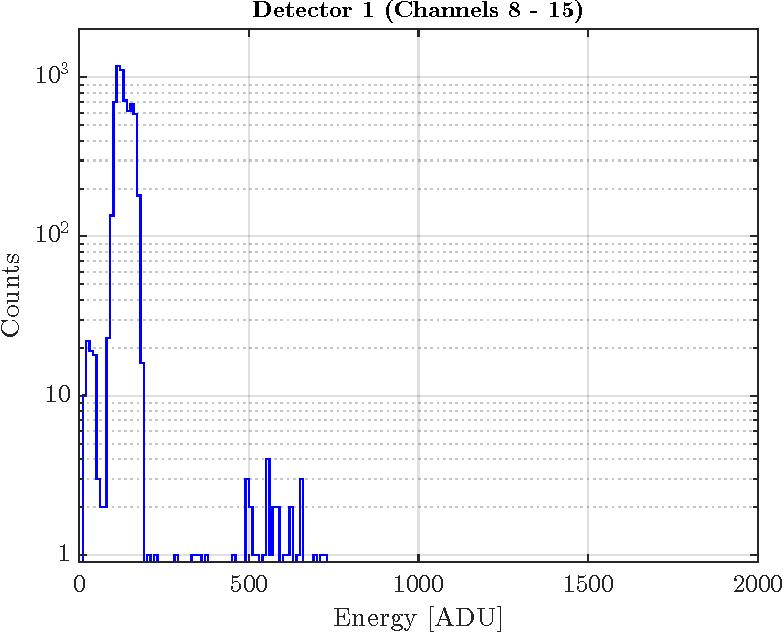
\includegraphics[width=0.475\textwidth]{Images/chap3/results/muons/ch_ext_trigger_4plots/incoming_energy34_2hr_sens2.pdf} & 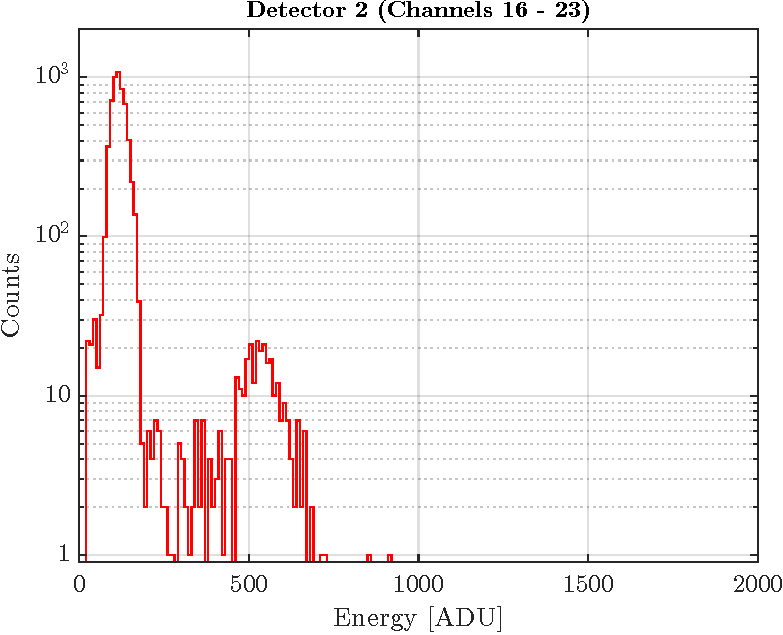
\includegraphics[width=0.475\textwidth]{Images/chap3/results/muons/ch_ext_trigger_4plots/incoming_energy34_2hr_sens3.pdf} \\
         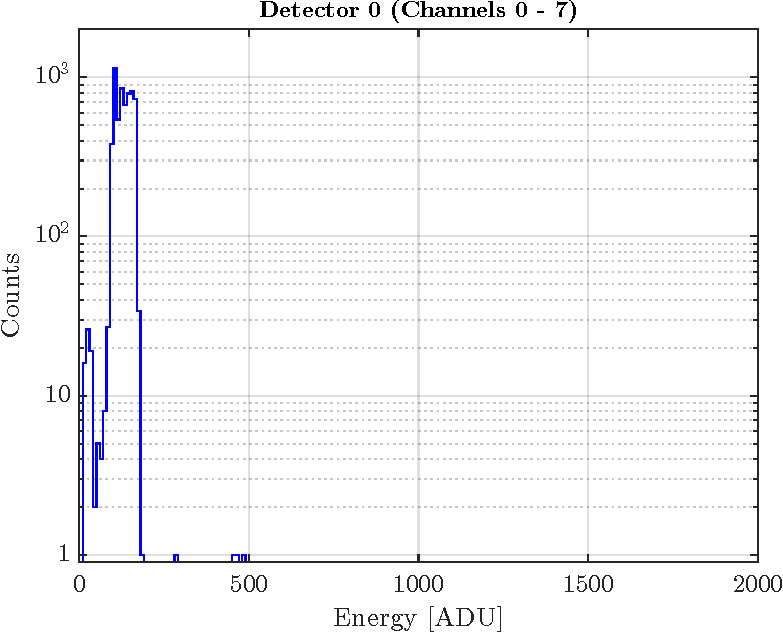
\includegraphics[width=0.475\textwidth]{Images/chap3/results/muons/ch_ext_trigger_4plots/incoming_energy34_2hr_sens1.pdf} & 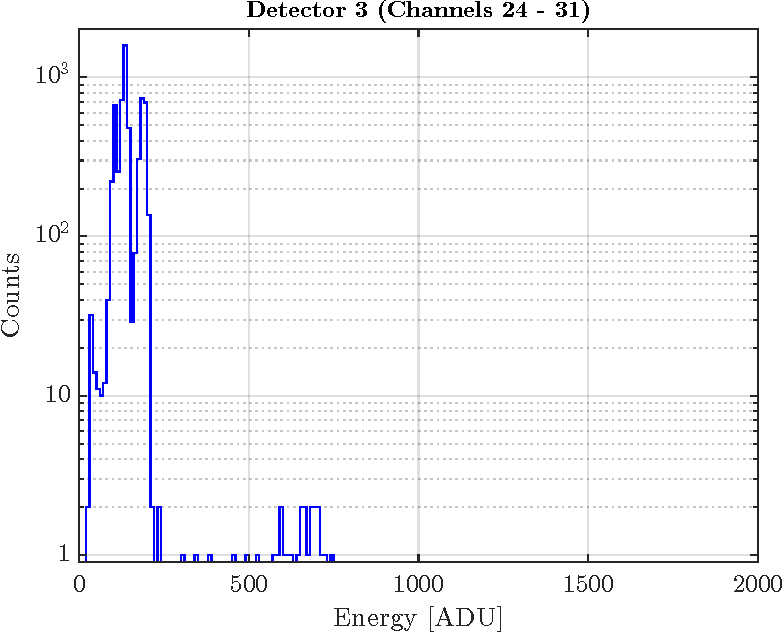
\includegraphics[width=0.475\textwidth]{Images/chap3/results/muons/ch_ext_trigger_4plots/incoming_energy34_2hr_sens4.pdf}
    \end{tabular}
    \caption{4 Si(Li) detectors view of a two-hour acquisition performed in external trigger mode with global threshold set to \texttt{130} and trigger hold delay set to 34 FPGA clocks. Channels from 16 to 23 are highlighted in red.}
    \label{figMUON4sensors}
\end{figure}

\par
The graph in \hyperref[figMUONselfExtComparativa]{Figure \ref{figMUONselfExtComparativa}} shows in pink the histogram associated with the acquisition performed in external trigger mode superimposed on the equivalent acquisition performed in self-trigger mode, considering in both cases the sum of the interaction events on all 32 channels. It can be seen that the energy peak in the muon region is lower in the external trigger measurement than in the self-trigger one.

\par
This phenomenon can be interpreted in two ways: first, the explanation could be associated therewith a geometrical aspect concerning the positioning of the scintillator with respect to the Si(Li) detector. In fact, the use of a single scintillator positioned below the sensor at a distance of  4 to \SI{5}{\cm} could result in the interaction with the scintillator of incident muons at an angle to the vertical greater than zero. This would result in the release of energy spread over several strips, so that a lower energy per strip is measured. To solve this problem, it would be necessary to use a second scintillator placed at a known distance from the first one, so that the trigger signal would be generated when an interaction event occurs on both scintillators. Such a device, based on the operating principle of a telescope, would make it possible to uniquely identify the interaction of vertically interacting muons with the Si(Li) detector, thus removing readings from the interaction with muons reaching the sensor at an angle from the vertical greater than zero.

% comparativa self external che evidenza ridotto picco energia muoni per external trigger: problema posizionamento o ritardo campionamento del canale
\begin{figure}[h!]
    \centering
    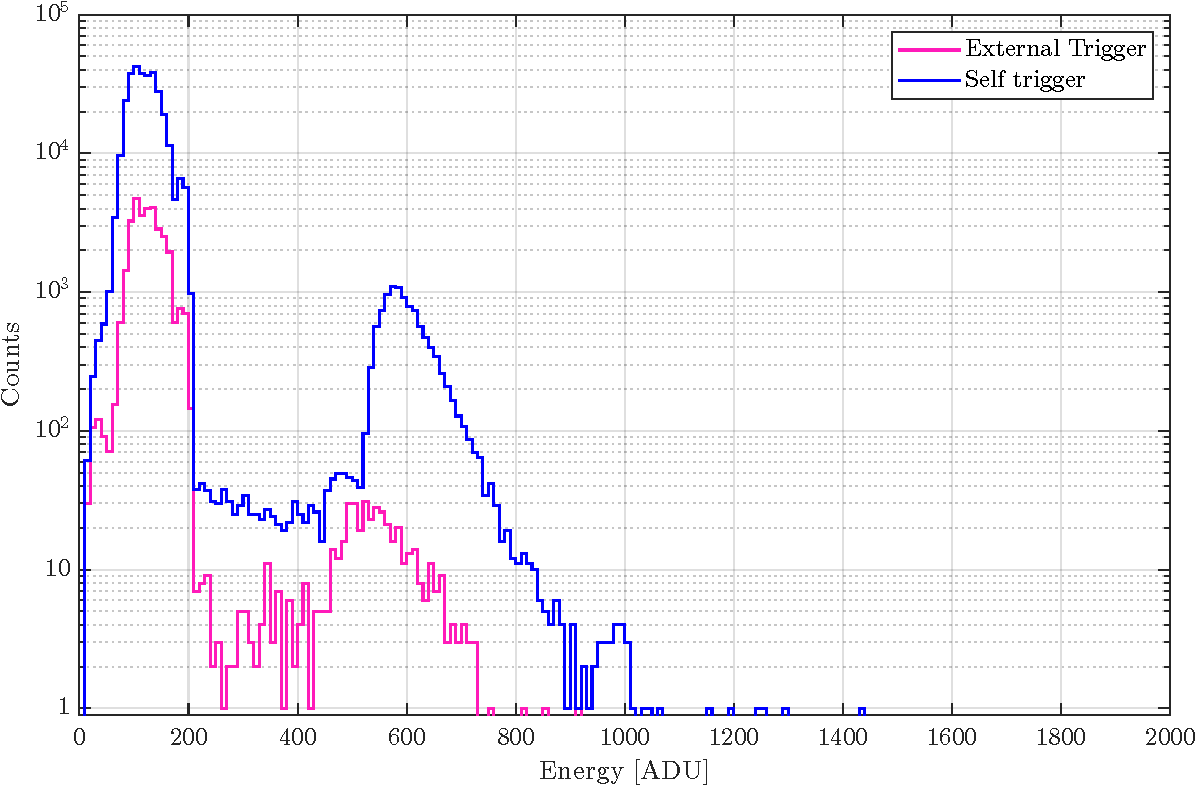
\includegraphics[width=0.75\textwidth]{Images/chap3/results/muons/incoming_energy_external34_self_100.pdf}
    \caption{Comparison between self trigger mode (in blue) and external trigger mode (in pink); both self and external trigger acquisitions were performed with global threshold set to \texttt{130} and trigger hold delay set to 34 FPGA clocks.}
    \label{figMUONselfExtComparativa}
\end{figure}

\par
A second hypothesis could be related to the time required for the ArduSiPM detector to generate the trigger signal. Indeed, it is possible that the time required for the detector to generate the trigger signal from the interaction event recorded in the scintillator is too long for the sample-and-hold circuit to sample the channel at the point of maximum signal output from the shaper filter. For this purpose, various delay values were evaluated, a parameter known as \textit{trigger hold delay}, which in the specific case of this test was set to 34 FPGA clocks. This parameter can be defined via the \texttt{GAPS\_DAQ} Python software and represents the delay, measured in FPGA clocks, that elapses from the acquisition of the trigger signal to the moment when the channel is actually sampled. With this trigger hold delay value, sampling may not occur at the maximum point of the signal output from the shaper, resulting in a lower recorded energy value than measured in self-trigger mode. 

\par
Unfortunately, it was not possible to measure by means of an oscilloscope the delay between the recording of the interaction event on the scintillator and the moment when the trigger signal is generated by the ArduSiPM device, shown in \hyperref[figArduiSiPMtrigger]{Figure \ref{figArduiSiPMtrigger}}. It is also possible that even a zero trigger hold delay value is not sufficient to ensure that the channel output is sampled at the correct instant, consistent with the set peak time \#4 ($\tau_{p} = \SI{0.98}{\micro\second}$), if the trigger generation delay is excessively high.

\begin{figure}[h!]
    \centering
    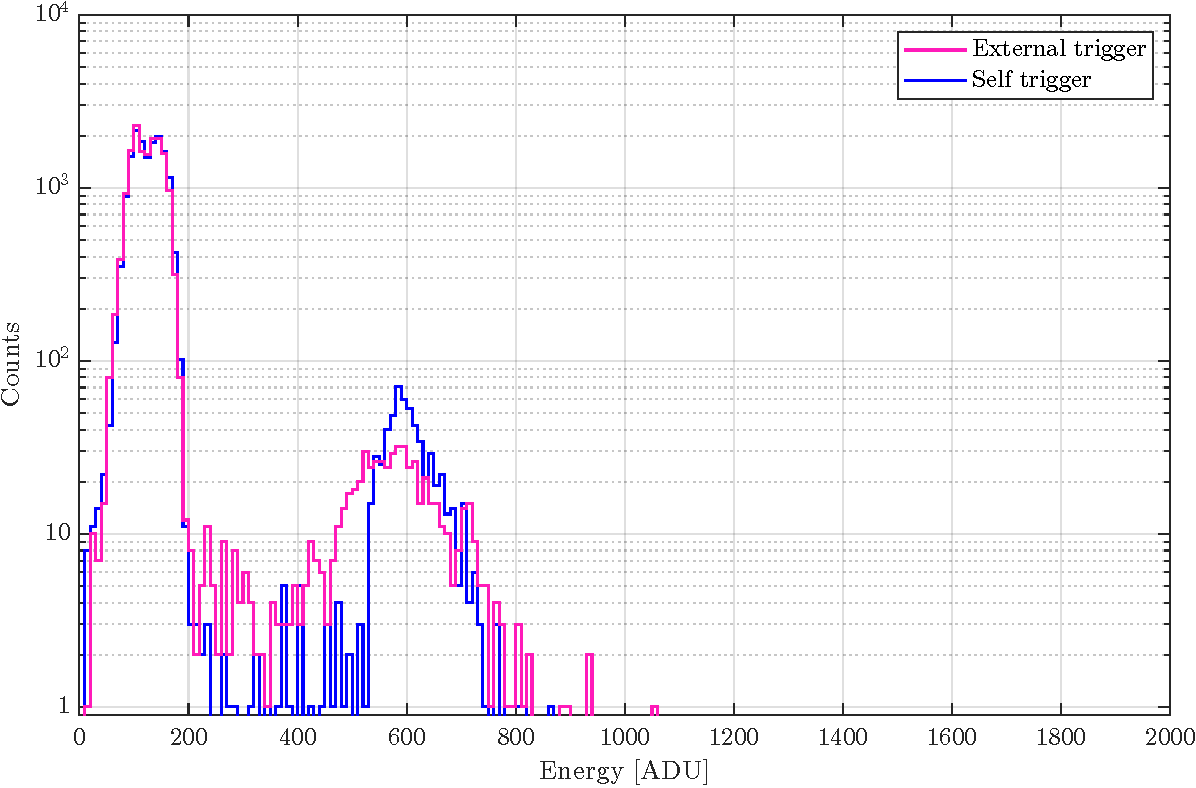
\includegraphics[width=0.75\textwidth]{Images/chap3/results/muons/ext_self_muons_THR_130_delay_34_ch0-7.pdf}
    \caption{Comparison between the measurement made in self-trigger mode (in blue) and that made in external trigger mode by placing the scintillator at a close distance from the Si(Li) detector (in red).}
    \label{figMUONselfExtComparativaCH0-7}
\end{figure}

\par
Further tests showed how the variation of the delay around the value used for the previous measurements varies the position of the muon peak in the external trigger measurements only slightly. On the contrary, it was ascertained how bringing the scintillator closer to the Si(Li) detector, in the order of a few millimetres instead of a few centimetres, resulted in the peak being shifted to higher energy, bringing it closer to that detected in the self-triggered acquisitions, as shown in the histogram presented in \hyperref[figMUONselfExtComparativaCH0-7]{Figure \ref{figMUONselfExtComparativaCH0-7}}. This leads to the conclusion that the phenomenon is mainly attributable to a geometric rather than a timing issue.